\documentclass{article}

\usepackage{amsmath,amsfonts,amssymb,amsthm}
\usepackage{thmtools}
\usepackage{stmaryrd}
\usepackage{natbib}
\usepackage{url}
\usepackage{array}
\usepackage{arydshln}
\usepackage{ifthen}
\usepackage{ifpdf}
\usepackage{verbatim}

\usepackage{mathtools}
\DeclarePairedDelimiter\ceil{\lceil}{\rceil}
\DeclarePairedDelimiter\floor{\lfloor}{\rfloor}

\usepackage{appendix}

\usepackage{tikz}
\usepackage{multirow}

\declaretheorem[numbered=yes,name=Lemma,qed=$\blacksquare$]{lemma}
\declaretheorem[numbered=yes,name=Definition,qed=$\blacksquare$]{definition}
\declaretheorem[numbered=yes,name=Specification,qed=$\blacksquare$]{specification}

\newcommand{\forcenewline}{$\phantom{v}$\\}

\newcommand{\update}[2]{[#1 \mapsto #2]}
\newcommand{\sem}[1]{\left\llbracket #1 \right\rrbracket}

%Math notation
\newcommand{\restrictfun}[1]{|_{#1}}
\newcommand{\parfun}{\rightharpoonup}
\newcommand{\finparfun}{\stackrel{\textit{\tiny{fin}}}{\rightharpoonup}}
\newcommand{\monnefun}{\stackrel{\textit{\tiny{mon, ne}}}{\longrightarrow}}
\newcommand{\monfun}{\stackrel{\textit{\tiny{mon}}}{\longrightarrow}}
\newcommand{\nefun}{\stackrel{\textit{\tiny{ne}}}{\longrightarrow}}
\newcommand{\fun}{\longrightarrow}
\newcommand{\defeq}{\stackrel{\textit{\tiny{def}}}{=}}
\newcommand{\nequal}[1][n]{\stackrel{\tiny{#1}}{=}}
\newcommand{\nsubeq}[1][n]{\stackrel{\tiny{#1}}{\subseteq}}
\newcommand{\nsupeq}[1][n]{\stackrel{\tiny{#1}}{\supseteq}}
\newcommand{\union}{\mathbin{\cup}}
\DeclareMathOperator{\dom}{dom}
\newcommand{\blater}{\mathop{\blacktriangleright}}
\newcommand{\id}{\var{id}}
\newcommand{\undefined}{\mathit{undefined}}

\newcommand{\powerset}[1]{\mathcal{P}(#1)}

\newcommand{\false}{\mathit{false}}
\newcommand{\true}{\mathit{true}}

%cofes
\newcommand{\cofe}{c.o.f.e.}
\newcommand{\cofes}{\cofe{}'s}
\newcommand{\CatC}{\mathbb{C}}
\newcommand{\CatP}{\mathbb{P}}

%Comments
\newcommand\lau[1]{{\color{purple} \sf \footnotesize {LS: #1}}\\}
\newcommand\dominique[1]{{\color{purple} \sf \footnotesize {DD: #1}}\\}
\newcommand\kars[1]{{\color{purple} \sf \footnotesize {LB: #1}}\\}

%Variables
\newcommand{\var}[1]{\mathit{#1}}
\newcommand{\hs}{\var{hs}}
\newcommand{\hv}{\var{hv}}
\newcommand{\rv}{\var{rv}}
\newcommand{\lv}{\var{lv}}
\newcommand{\pc}{\mathit{pc}}
\newcommand{\pcreg}{\mathrm{pc}}
\newcommand{\addr}{\var{a}}
\newcommand{\offset}{\var{offset}}
\newcommand{\word}{\var{w}}
\newcommand{\start}{\var{base}}
\newcommand{\addrend}{\var{end}}
\newcommand{\mem}{\var{mem}}
\newcommand{\reg}{\var{reg}}
\newcommand{\heapseg}{\var{hs}}
\newcommand{\heap}{\var{heap}}
\newcommand{\mode}{\var{mode}}
\newcommand{\perm}{\var{perm}}
\newcommand{\roll}{\var{roll}}
\newcommand{\instr}{\var{instr}}

\newcommand{\stdcap}[1][\perm]{\left(#1,\start,\addrend,\addr \right)}

%Memory projections
\newcommand{\plainproj}[1]{\mathrm{#1}}
\newcommand{\memheap}[1][\Phi]{#1.\plainproj{heap}}
\newcommand{\memreg}[1][\Phi]{#1.\plainproj{reg}}

\newcommand{\updateHeap}[3][\Phi]{#1\update{\plainproj{heap}.#2}{#3}}
\newcommand{\updateReg}[3][\Phi]{#1\update{\plainproj{reg}.#2}{#3}}

%Configuration end states
\newcommand{\failed}{\textsl{failed}}
\newcommand{\halted}{\textsl{halted}}

%Functions
\newcommand{\plainfun}[2]{
  \ifthenelse{\equal{#2}{}}
             {\mathit{#1}}
             {\mathit{#1}(#2)}
}
\newcommand{\decode}{\plainfun{decode}{}}
\newcommand{\encode}{\plainfun{encode}{}}
\newcommand{\encodePerm}{\plainfun{encodePerm}{}}
\newcommand{\updatePcPerm}[1]{\plainfun{updatePcPerm}{#1}}

\newcommand{\executeAllowed}[1]{\plainfun{executeAllowed}{#1}}
\newcommand{\nonZero}[1]{\plainfun{nonZero}{#1}}
\newcommand{\readAllowed}[1]{\plainfun{readAllowed}{#1}}
\newcommand{\writeAllowed}[1]{\plainfun{writeAllowed}{#1}}
\newcommand{\withinBounds}[1]{\plainfun{withinBounds}{#1}}
\newcommand{\stdUpdatePc}[1]{\plainfun{updatePc}{#1}}

\newcommand{\readCond}[1]{\plainfun{readCondition}{#1}}
\newcommand{\writeCond}[1]{\plainfun{readWriteCondition}{#1}}
\newcommand{\execCond}[1]{\plainfun{executeCondition}{#1}}
\newcommand{\entryCond}[1]{\plainfun{entryCondition}{#1}}


%World operations
\newcommand{\future}{\mathbin{\sqsupseteq}}
\newcommand{\heapSat}[3][\heap]{#1 :_{#2} #3}

%Assembly labels
\newcommand{\codelabel}[1]{\mathit{#1}}
\newcommand{\init}{\codelabel{init}}
\newcommand{\malloc}{\codelabel{malloc}}
\newcommand{\counter}{\codelabel{counter}}
\newcommand{\iocap}{\codelabel{iocap}}

%Type(s)
\newcommand{\type}[1]{\mathrm{#1}}
\newcommand{\asmType}{\plaindom{AsmType}}


%Domains
\newcommand{\plaindom}[1]{\mathrm{#1}}
\newcommand{\Caps}{\plaindom{Cap}}
\newcommand{\Words}{\plaindom{Word}}
\newcommand{\Addrs}{\plaindom{Addr}}
\newcommand{\Mems}{\plaindom{Mem}}
\newcommand{\RegName}{\plaindom{RegisterName}}
\newcommand{\Regs}{\plaindom{Reg}}
\newcommand{\Heaps}{\plaindom{Heap}}
\newcommand{\HeapSegments}{\plaindom{HeapSegment}}
\newcommand{\Confs}{\plaindom{Conf}}
\newcommand{\Instrs}{\plaindom{Instructions}}
\newcommand{\nats}{\mathbb{N}}
\newcommand{\ints}{\mathbb{Z}}
\newcommand{\Perms}{\plaindom{Perm}}

\newcommand{\Rel}{\plaindom{Rel}}
\newcommand{\States}{\plaindom{State}}
\newcommand{\RegionNames}{\plaindom{RegionName}}
\newcommand{\Regions}{\plaindom{Region}}
\newcommand{\Worlds}{\plaindom{World}}
\newcommand{\Wor}{\plaindom{Wor}}
\newcommand{\StorePred}{\plaindom{HeapSegPred}}
\newcommand{\UPred}[1]{\plaindom{UPred}(#1)}

%LR
\newcommand{\intr}[2]{\mathcal{#1}}
\newcommand{\valueintr}[1]{\intr{V}{#1}}
\newcommand{\exprintr}[1]{\intr{E}{#1}}
\newcommand{\contintr}[1]{\intr{K}{#1}}
\newcommand{\regintr}[1]{\intr{R}{#1}}
\newcommand{\stdvr}{\valueintr{\asmType}}
\newcommand{\stder}{\exprintr{\asmType}}
\newcommand{\stdrr}{\regintr{\asmType}}
\newcommand{\stdkr}{\contintr{\asmType}}
\newcommand{\observations}{\mathcal{O}}
\newcommand{\npair}[2][n]{\left(#1,#2 \right)}

%Reference register/heap
\newcommand{\refreg}[1]{\lfloor #1 \rfloor}
\newcommand{\refheap}[1]{\langle #1 \rangle_h}

%Instructions
%No arguments
\newcommand{\zinstr}[1]{\mathtt{#1}}
\newcommand{\fail}{\zinstr{fail}}
\newcommand{\halt}{\zinstr{halt}}
%One argument
\newcommand{\oneinstr}[2]{\zinstr{#1} \; #2}
\newcommand{\jmp}[1]{\oneinstr{jmp}{#1}}
%Two arguments
\newcommand{\twoinstr}[3]{\zinstr{#1} \; #2 \; #3}
\newcommand{\jnz}[2]{\twoinstr{jnz}{#1}{#2}}
\newcommand{\isptr}[2]{\twoinstr{isptr}{#1}{#2}}
\newcommand{\setptr}[2]{\twoinstr{setptr}{#1}{#2}}
\newcommand{\move}[2]{\twoinstr{move}{#1}{#2}}
\newcommand{\store}[2]{\twoinstr{store}{#1}{#2}}
\newcommand{\load}[2]{\twoinstr{load}{#1}{#2}}
\newcommand{\lea}[2]{\twoinstr{lea}{#1}{#2}}
%Three arguments
\newcommand{\threeinstr}[4]{\zinstr{#1} \; #2 \; #3 \; #4}
\newcommand{\restrict}[3]{\threeinstr{restrict}{#1}{#2}{#3}}
\newcommand{\subseg}[3]{\threeinstr{subseg}{#1}{#2}{#3}}
\newcommand{\plus}[3]{\threeinstr{plus}{#1}{#2}{#3}}

%Permissions
\newcommand{\plainperm}[1]{\mathrm{#1}}
\newcommand{\noperm}{\plainperm{o}}
\newcommand{\readonly}{\plainperm{ro}}
\newcommand{\readwrite}{\plainperm{rw}}
\newcommand{\exec}{\plainperm{rx}}
\newcommand{\entry}{\plainperm{e}}
\newcommand{\rwx}{\plainperm{rwx}}

%OP sem
\newcommand{\diverge}[1][n]{\not\Downarrow_{#1}}
\newcommand{\step}[1][]{\rightarrow_{#1}}

\begin{document}
\begin{flushright}
\today
\end{flushright}
$\RegName$ contains $\pcreg$, but is otherwise some undefined, finite set.
\begin{align*}
\Addrs &::= \nats & & &
\Words &::= \Caps + \ints \\
\Regs  &::= \RegName \rightarrow \Words & & &
\Heaps &::= \Addrs \rightarrow \Words \\
\Perms &::= \{ \noperm, \readonly, \readwrite, \exec, \entry, \rwx\} & & &
\Mems  &::= \Regs \times \Heaps \\
\Caps  &::= \Perms \times \Addrs \times \Addrs \times \Addrs & & &
\Confs &::= \Mems + \{\failed, \halted \times \Mems\} \\
\HeapSegments &::= \Addrs \parfun \Words & & & &
\end{align*}

\begin{figure}[!h]
  \centering
  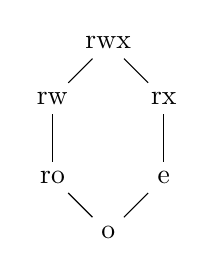
\begin{tikzpicture}[main node/.style={}]
  \node[main node] (1) {$\rwx$};
  \node[main node] (2) [below right of=1] {$\exec$};
  \node[main node] (3) [below of=2] {$\entry$};
  \node[main node] (4) [below left of=1] {$\readwrite$};
  \node[main node] (5) [below of=4] {$\readonly$};
  \node[main node] (6) [below right of=5] {$\noperm$};

  \path[every node/.style={font=\sffamily\small}]
    (1) edge (2)
    (2) edge (3)
    (3) edge (6)
    (1) edge (4)
    (4) edge (5)
    (5) edge (6);
\end{tikzpicture}
\caption{Permission hierarchy}
\label{fig:perm-hier}
\end{figure}
Notation:
$$\begin{array}{rcl}
i       &\in& \Instrs \\
r       &\in& \RegName\\
\mem    &::=& (\reg,\heap)\\
\pc     &\in& \Caps \\
\pcreg  &\in& \RegName \\
\Phi    &::=& \mem \in \Confs\\
\memheap&\in& \Heaps \\
\memreg &\in& \Regs \\
\addr   &\in& \Addrs\\
\perm   &\in& \Perms\\
(\perm,\start,\addrend,\addr) &\in& \Caps \\
n       &\in& \ints\\
\end{array}$$
Further definitions:
$$\begin{array}{rcl}
\lv    &::=& \refreg{r} \\
\hv    &::=& \refheap{r}\\
\rv    &::=& n \mid \lv \\
i      &::=& \fail \mid \halt \mid 
             \jmp{\lv} \mid \jnz{\lv}{\rv} \mid
             \isptr{\lv}{\rv} \mid \setptr{\lv}{\rv} \mid \\
       &   & \lea{\lv}{\rv} \mid\move{\lv}{\rv} \mid \load{\lv}{\hv} \mid \store{\hv}{\rv} \mid  \\
       &   & \restrict{\lv}{\rv}{\rv} \mid \subseg{\lv}{\rv}{\rv} \mid \plus{\lv}{\rv}{\rv}
\end{array}$$

\subsection*{Semantics}
Assume a $\decode$ function that decodes integer to instructions:
\begin{align*}
\decode &:\Words \rightarrow \Instrs
\end{align*}
Assume an $\encodePerm$ function that encodes a permission as an integer:
\begin{align*}
\encodePerm &: \Perms \rightarrow \ints
\end{align*}
\begin{align*}
  \Phi & \rightarrow \sem{\decode(\memheap(\addr))}(\Phi) & &                                   
                                                              \arraycolsep=0pt
                                                              \begin{array}{l}
                                                                \text{if $\memreg(\pcreg) = \stdcap$}\\
                                                                \quad\text{and $\start \leq \addr < \addrend$}\\
                                                                \quad\text{and $\perm \in \{ \exec,\rwx \}$ }
                                                              \end{array}\\
\Phi & \rightarrow \failed                                 & & \text{otherwise}
\end{align*}
It is assumed that address 0 is used for I/O, so whatever resides in location 0 after an execution can be seen as a result. As we will see in the semantics, it is assumed that the initial process starts with a readwrite capability for this location.
\begin{align*}
  \executeAllowed{\perm} &=
                           \begin{cases}
                             \true & \text{if } \perm \in \{ \rwx, \exec, \entry \} \\
                             \false & \text{otherwise}
                           \end{cases} \\
  \readAllowed{\perm} &=
                           \begin{cases}
                             \true & \text{if } \perm \in \{ \rwx, \exec, \readwrite, \readonly \} \\
                             \false & \text{otherwise}
                           \end{cases} \\
  \writeAllowed{\perm} &=
                           \begin{cases}
                             \true & \text{if } \perm \in \{ \rwx, \readwrite\} \\
                             \false & \text{otherwise}
                           \end{cases} \\
  \updatePcPerm{(\perm,\start,\addrend,\addr)} &=
                                     \begin{cases}
                                       (\exec,\start,\addrend,\addr) & \text{if $\perm = \entry$}\\
                                       (\perm,\start,\addrend,\addr) & \text{otherwise} 
                                     \end{cases} \\
  \nonZero{w} &=
                \begin{cases}
                  \true & \text{if $w\in \Caps$ or $w\in \ints$ and $w \neq 0$}\\
                  \false & \text{otherwise}
                \end{cases} \\
  \withinBounds{(\_,\start,\addrend,\addr)} &=
                                              \begin{cases}
                                                \true  & \text{if $\start \leq \addr \leq \addrend$} \\
                                                \false & \text{otherwise}
                                              \end{cases} \\
  \stdUpdatePc{\Phi} &=
                       \begin{cases}
                         \updateReg{\pcreg}{\var{newPc}} & 
                           \arraycolsep=0pt
                           \begin{array}{l}
                             \text{if $\memreg(\pcreg) = \stdcap$}\\
                             \quad\text{and $\var{newPc} = (\perm,\start,\addrend,\addr + 1)$}\\
                           \end{array} \\
                           \failed & \text{otherwise}
                       \end{cases} \\
\end{align*}
%TODO: \Phi.reg(rv) to some other notation. It should only look up reg, if it is a regname otherwise just the litteral.
\begin{align*}
  \sem{\fail}(\Phi)                        & = \failed \\
  \sem{\halt}(\Phi)                        & = (\halted,\Phi) \\
  \sem{\jmp{\lv}}(\Phi)                    & = \updateReg{\pcreg}{\updatePcPerm{\memreg(\lv)}} \\
  \sem{\jnz{\lv}{\rv}}(\Phi)               & = 
                                             \begin{cases}
                                               \updateReg{\pcreg}{\updatePcPerm{\memreg(\lv)}} &
                                               \arraycolsep=0pt
                                               \begin{array}{l}
                                                 \text{if $\nonZero{\memreg(\rv)}$} 
                                               \end{array}\\
                                               \stdUpdatePc{\Phi} & \text{if not $\nonZero{\memreg(\rv)}$}\\
                                               \failed & \text{otherwise }
                                             \end{cases} \\
 \sem{\load{\refreg{r_1}}{\refheap{r_2}}}  & = 
                                             \begin{cases}
                                               \stdUpdatePc{\updateReg{r_1}{\var{w}}} &
                                               \arraycolsep=0pt
                                               \begin{array}{l}
                                                 \text{if }\memreg(r_2) = (\perm,\start,\addrend,\addr) = \var{c} \\
                                                 \quad\text{and }\readAllowed{\perm} \text{ and } \withinBounds{\var{c}} \\
                                                 \quad\text{and }\var{w} = \memheap(\addr)
                                               \end{array}\\
                                               \failed & \text{otherwise }
                                             \end{cases}\\
 \sem{\store{\refheap{r_1}}{\refreg{r_2}}} & = 
                                             \begin{cases}
                                               \stdUpdatePc{\updateHeap{\addr}{\var{w}}} &
                                               \arraycolsep=0pt
                                               \begin{array}{l}
                                                 \text{if }\memreg(r_1) = (\perm,\start,\addrend,\addr) = \var{c} \\
                                                 \quad\text{and }\writeAllowed{\perm} \text{ and } \withinBounds{\var{c}} \\
                                                 \quad\text{and }\var{w} = \memreg(r_2)
                                               \end{array}\\
                                               \failed & \text{otherwise }
                                             \end{cases}\\
 \sem{\move{\refreg{r_1}}{\rv}}            & = \stdUpdatePc{\updateReg{r_1}{\memreg(\rv)}}
\\
  \sem{\lea{\refreg{r_1}}{\rv}}            & =
                                             \begin{cases}
                                               \stdUpdatePc{\updateReg{r_1}{\var{c}}} &
                                                 \arraycolsep=0pt
                                                 \begin{array}{l}
                                                   \text{if either $n = \rv$ or $\rv = \refreg{r_2}$ and $n = \memreg(r_2)$} \\
                                                   \quad\text{and in either case $n \in \ints $} \\
                                                   \quad\text{and $\memreg(r_1) = \stdcap$}\\
                                                   \quad\text{and $\var{c} = (\perm,\start,\addrend,\addr + n)$}
                                                 \end{array}\\
                                               \failed               & \text{otherwise}
                                             \end{cases} 
\\
 % In the M-Machine, lea checks whether the pointer stay within the allowed range in the pointer.
  \sem{\restrict{\refreg{r_1}}{\rv_1}{\rv_2}}           & =
                                             \begin{cases}
                                               \stdUpdatePc{\updateReg{r_1}{\var{c}}}  &
                                                 \arraycolsep=0pt
                                                 \begin{array}{l}
                                                   \text{if $\memreg(\rv_1) = c'$}\\
                                                   \quad\text{and $c' = \stdcap$}\\
                                                   \quad\text{and either $\rv_2 = n$ or $\memreg(\rv_2) = n$}\\
                                                   \quad\text{and in either case $n \in \ints$}\\
                                                   \quad\text{and $\var{newPerm} = \encodePerm(n)$}\\
                                                   \quad\text{and $\var{newPerm} \sqsubseteq \perm$}\\
                                                   \quad\text{and $c = (\var{newPerm},\start,\addrend,\addr)$}
                                                 \end{array}\\
                                               \failed                   & \text{otherwise}
                                             \end{cases} 
\end{align*}
\begin{align*}
  \sem{\plus{\refreg{r_1}}{\rv_1}{\rv_2}}               & =
                                                          \begin{cases}
                                                            \stdUpdatePc{\updateReg{r_1}{n_1+n_2}} &
                                                            \arraycolsep=0pt
                                                            \begin{array}{l}
                                                              \text{if for $i \in \{1,2\}$}\\
                                                              \quad\text{$n_i = \rv_i$ or $n_i = \memreg{\rv_i}$}\\
                                                              \quad\text{and in either case $n_i \in \ints$}
                                                            \end{array}\\
                                                            \failed & \text{otherwise}
                                                          \end{cases}\\
  \sem{\isptr{\lv}{\rv}} & = \undefined \\ 
  \sem{\setptr{\lv}{\rv}} & = \undefined \\ 
  \sem{\subseg{\lv}{\rv}{\rv}} & = \undefined 
\end{align*}

\section{Examples}
\label{sec:examples}
\subsection{Ticket Dispenser}
\label{sec:tick-disp}
\newcommand{\hsfoot}{\hs_\var{footprint}}
\newcommand{\hsframe}{\hs_\var{frame}}
\newcommand{\size}{\var{size}}
\newcommand{\rio}{r_{io}}
\newcommand{\adv}{\codelabel{adv}}
\newcommand{\advb}{\var{adv_{base}}}
\newcommand{\adve}{\var{adv_{end}}}
\newcommand{\initb}{\var{init}_{base}}
\newcommand{\inite}{\var{init}_{end}}
\newcommand{\mrlen}{5cm}
\newcommand{\retm}{\var{ret}_{\malloc}}
\newcommand{\reta}{\var{ret}_{\adv}}
\newcommand{\base}{\var{base}}
\newcommand{\eend}{\var{end}}
\newcommand{\bracket}[1]{\multirow{#1}{*}{\ensuremath{
 \left . \vphantom{\begin{array}{l}
 \ifthenelse{\equal{#1}{1}}{3\\}{
    \ifthenelse{\equal{#1}{2}}{3\\3\\}{
    \ifthenelse{\equal{#1}{3}}{3\\3\\3\\}{
    \ifthenelse{\equal{#1}{4}}{3\\3\\3\\3\\}{
    \ifthenelse{\equal{#1}{5}}{3\\3\\3\\3\\3\\}{
    \ifthenelse{\equal{#1}{6}}{3\\3\\3\\3\\3\\3\\}{
      3\\3\\3\\3\\3\\3\\3\\ %7
  }}}}}}
  \end{array}} \right \}}}
}
\newcommand{\annotate}[2]{\multirow{#1}{\mrlen}{\scriptsize #2}}
Assume the instructions of some adversary resides in the memory starting at the memory location marked with $\advb$. Assume that the register $\rio$ initially contains a capability for the address in memory where I/O is written to (we assume this address is 0). We assume that entry capabilities for $\adv$ and $\malloc$ is ambiently available\dominique{what does this mean?}. The following is a test program for a ticket dispenser:
\[
  \begin{array}{r l l p{\mrlen}}
% Set io to -1
\initb:     & \store{\refheap{\rio}}{-1} & \bracket{1} & \annotate{1}{Initialize io to $-1$} \\
% Store io capability just after jump to adv
           & \move{\refreg{r_0}}{\refreg{\pcreg}} & \bracket{3} & \annotate{3}{Store the io capability on the stack} \\
           & \lea{\refreg{r_0}}{\iocap} & & \\
           & \store{\refheap{r_0}}{\refreg{\rio}} & & \\
% Overwrite io register
           & \move{\refreg{\rio}}{0} & \bracket{1} & \annotate{1}{Overwrite io register} \\
% Allocate memory for ticket dispenser program
           & \move{\refreg{r_1}}{\size} &  \bracket{4} & \annotate{4}{Allocate memory for the ticket dispenser program (including memory for counter and capability for counter)}\\
           & \move{\refreg{r_0}}{\refreg{\pcreg}} & & \\
           & \lea{\refreg{r_0}}{3} & & \\
           & \jmp{\malloc} & & \\
% Save ticket dispenser code
\retm:     & \store{\refheap{r_1}}{(\encode(i_1))} & \bracket{7} & \annotate{7}{Store the ticket dispenser program in the newly allocated memory} \\
           & \lea{\refreg{r_1}}{1} & & \\
           & \store{\refheap{r_1}}{(\encode(i_2))} & & \\
           & \lea{\refreg{r_1}}{1} & & \\
           & \vdots & & \\
           & \store{\refheap{r_1}}{(\encode(i_7))} & & \\
           & \lea{\refreg{r_1}}{1} & & \\
% Save capability for counter
           & \move{\refreg{r_0}}{\refreg{r_1}} & \bracket{4} & \annotate{4}{Store a capability for the counter address after the ticket dispenser program} \\
           & \lea{\refreg{r_0}}{1} & & \\
           & \store{\refheap{r_1}}{\refreg{r_0}} & & \\
           & \lea{\refreg{r_1}}{1} & & \\
% Save capability for counter two addresses after jump to adv.
           & \move{\refreg{r_2}}{\refreg{\pcreg}} & \bracket{3} & \annotate{3}{Store a capability for the counter in this code} \\
           & \lea{\refreg{r_2}}{\counter} & & \\
           & \store{\refheap{r_2}}{r_0} & & \\
           & \move{\refreg{r_2}}{0} & \bracket{1} & \annotate{1}{Overwrite capability for counter} \\
% Save counter
           & \store{\refheap{r_1}}{0} & \bracket{1} & \annotate{1}{Initialize counter to 0} \\
% Change pointer to point to start of ticket dispenser code
           & \lea{\refreg{r_1}}{-8} & \bracket{1} & \annotate{1}{Capability points to start of td code \footnote{This is also the argument for the adversary}} \\
% Set up entry pointer to ticketDispenser for adv.
           & \restrict{\refreg{r_1}}{\refreg{r_1}}{(\encodePerm{(\entry)})} &\bracket{1} & \annotate{1}{Restrict cap. to td} \\
% Set up return pointer
           & \move{\refreg{r_0}}{\refreg{\pcreg}} & \bracket{3} & \annotate{3}{Setup a return pointer for the adversary} \\
           & \lea{\refreg{r_0}}{5} & & \\
           & \restrict{\refreg{r_0}}{\refreg{r_0}}{(\encodePerm{(\entry)})} & & \\
% jump to adv
           & \jmp{\adv} & \bracket{1} & \annotate{1}{Jump to the adversary} \\
           & 0 & \bracket{1} & \annotate{1}{Address reserved for io cap.} \\
           & 0 & \bracket{1} & \annotate{1}{Address reserved for counter cap.} \\
% retrieve io capability
\reta:     & \move{\refreg{r_0}}{\refreg{\pcreg}} & \bracket{3} & \annotate{3}{Retrieve the io capability} \\
           & \lea{r_0}{-2} & & \\
           & \load{\refreg{\rio}}{\refheap{r_0}} & & \\
% retieve counter capability
           & \lea{r_0}{1} & \bracket{2} & \annotate{2}{Retrieve the counter capability} \\
           & \load{\refreg{r_1}}{\refheap{r_0}} & & \\
% load the value of the counter
           & \load{\refreg{r_0}}{\refheap{r_1}} & \bracket{2} & \annotate{2}{Read the counter and write it to io address} \\
% store the value of the counter to io
           & \store{\refheap{\rio}}{\refreg{r_0}} & & \\
\inite :   & \halt
  \end{array}
\]
Here $\size$ is 9. The variables $\counter$ and $\iocap$ are respectively the offsets to the addresses reserved for the counter and io capabilities. $i_1 \dots i_7$ refers to the instructions in the following ticket dispenser:
\[
  \begin{array}{r l}
    i_1 :& \move{\refreg{r_2}}{\refreg{\pcreg}} \\
    i_2 :& \load{\refreg{r_2}}{\size - 2} \\
    i_3 :& \load{\refreg{r_1}}{\refheap{r_2}}\\
    i_4 :& \plus{\refreg{r_3}}{\refreg{r_1}}{2} \\
    i_5 :& \store{\refheap{r_2}}{\refreg{r_3}} \\
    i_6 :& \move{\refreg{r_2}}{0} \\
    i_7 :& \jmp{\refreg{r_0}}
  \end{array}
\]
The heap layout for the above program can be seen in Figure~\ref{tab:tick-disp-heap}.
\begin{figure}[ht]
  \centering
  \begin{tabular}{ | c | l | }
    \hline
    Addr. & Content \\ \hline
    0   &  $i_1$ \\ \hline
    1   &  $i_2$ \\ \hline
    2   &  $i_3$ \\ \hline
    3   &  $i_4$ \\ \hline
    4   &  $i_5$ \\ \hline
    5   &  $i_6$ \\ \hline
    5   &  $i_7$ \\ \hline
    7   & Cap. for addr. 8 \\ \hline
    8   & The counter \\ \hline  
  \end{tabular}
  \caption{The heap layout for the ticket dispenser.}
  \label{tab:tick-disp-heap}
\end{figure}

In the JS paper, the ticket dispenser program dereferences the counter and returns the value. It does not seem like a similar thing would work here as the adversary can do even more. In particular, the adversary can execute a $\halt$ instruction that will cause the machine to halt (successfully). The adversary could also choose never to return to the return address that we set up for him.
\begin{lemma}[Ticket dispenser test]\dominique{I would prefer more precise, symbolic statements of assumptions and less prose.}
\label{lem:tckt-disp}
 Given a configuration $\Phi$, if
 \begin{description}
 \item[$\boldsymbol \memheap$] contains the ticket dispenser test program starting at the address labelled $\initb$, 
 \item[$\boldsymbol \memheap$] contains the adversary code starting at label $\advb$. The adversary is assumed to have no capabilities on the heap, but it has access to the ambient $\malloc$ capability! \lau{maybe mention that malloc is also on the heap}
 \item[$\boldsymbol \memheap$] contains the malloc code, and the malloc code satisfy $\iota_{\malloc}$, i.e., $\forall n \ldotp \heapSat[{\heap\restrictfun{\{\malloc_{\var{base}}, \dots ,\malloc_{\var{end}}\}}}]{n}{W_{\malloc}}$.
 \item[All the above programs are disjoint.]
 \item[$\boldsymbol{\adv}$ and $\boldsymbol{ \codelabel{malloc}}$] capabilities are ambiently available at all times.
 \item[$\boldsymbol{ \memreg(\pcreg)}$] is $(\rwx,\initb,\inite,\initb)$.
 \item[$\boldsymbol{ \memreg(\rio)}$] is $(\readwrite,0,0,0)$.
 \item[the remaining registers] all contains 0,
 \end{description}
 and $\Phi \rightarrow^* (\halted,\Phi')$, then the I/O address (that is $\memheap[\Phi'](0)$) contains either $-1$ or a number that is $\geq 0$ and even.
\end{lemma}
In the initial configuration the $\pcreg$ register is assumed to have an execute and write permission for the area of the heap where the program resides.

The ticket dispenser test program uses $\malloc$. To be able to reason about programs that use $\malloc$, we assume that it follows the following specification. If you provide it with one argument, namely the size of the allocation you wish and a return capability, then at some point $\pcreg$ will contain an executable capability based on this return capability and the return register will contain a $\rwx$ capability for the freshly allocated memory. 
\begin{specification}[Malloc v.2]
  \begin{align*}
    &\forall \Phi \in \Mems \ldotp \forall \hsfoot, \hsframe \in \HeapSegments \ldotp \\
    &\quad \forall n, \size \in \nats \ldotp \forall b,e,a,m_b,m_e \in \Addrs\ldotp\forall p \in \Perms \ldotp \forall W \in \Worlds \ldotp\\
    &\qquad \exists i, \iota_{\malloc} \ldotp \\
    &\qquad \quad W = [i \mapsto \iota_{\malloc}] \land \\
    &\qquad \quad \dom(\hsfoot) = [m_b,m_e] \land \\ % This
    &\qquad \quad \memheap = \hsfoot \uplus \hsframe \land\\
    &\qquad \quad \heapSat[\hsfoot]{n}{W} \land \\
    &\qquad \quad \memreg(r_1) = \size \land \\
    &\qquad \quad \size \geq 0 \land \\
    &\qquad \quad \memreg(r_0) = (p,b,e,a) \land \\
    &\qquad \quad \memreg(\pcreg) = (\entry,m_b,m_e,m_b) \\ %and this needs to change with ABI.
    &\qquad \quad \Rightarrow \\
    &\qquad \qquad\exists \Phi' \in \Mems \ldotp \exists \hsfoot' \in \HeapSegments\ldotp\\
    &\qquad \qquad \quad \exists j,k \in \nats \ldotp \exists b',e'\in \Addrs \ldotp \exists W' \in \Worlds \ldotp \\
    &\qquad \qquad \qquad \Phi \step[j]\Phi' \land \\
    &\qquad \qquad \qquad \memheap[\Phi']=\hsfoot' \uplus \hsframe \land\\
    &\qquad \qquad \qquad W' = [k \mapsto \iota_{b',e'}^0, i \mapsto \iota_{\malloc}]\\
    &\qquad \qquad \qquad W' \future W \land \\
    &\qquad \qquad \qquad \heapSat[\hsfoot']{n-j}{W'} \land \\
    &\qquad \qquad \qquad \memreg[\Phi'](\pcreg) = (\updatePcPerm{p},b,e,a) \land \\
    &\qquad \qquad \qquad \size = e'-b' \\
    &\qquad \qquad \qquad \memreg[\Phi'](r_1) = (\rwx,b',e',b') \land \\
    &\qquad \qquad \qquad \forall r \in \RegName \setminus \{\pcreg,r_1\} \ldotp \memreg[\Phi'](r) = 0
  \end{align*}
\end{specification}
The specification uses the malloc island defined as
\lau{I am not satisfied with the pc in the premise. The exact capability necessary very much depend on the implementation (this is mostly a note to myself.)}
\dominique{I agree with the remark about the pc.  Perhaps leave the form of the
  pc unspecified as it is not important for malloc users?}
\dominique{Resulting frame should be equal to original.}
\lau{Rewrite the specification when we have settled on a reasonable way to handle ABI.}

\begin{specification}[Malloc]\dominique{can you state this more systematically, with less prose, more explicit assumptions and conclusion?}
Take $W_{\malloc}$ the world with exactly one island, namely the unspecified island $\iota_{\malloc}$ that governs the internal state of $\malloc$.  If we invoke $\malloc$ in a memory $h = \hsframe \uplus \hsfoot$
%\lau{Is $\hsframe$ supposed to be the rest of memory, so $h$ is something we can execute in? Is $\malloc$ allowed to allocate more memory, i.e., how does $\hsfoot$ relate to $\hsfoot'$?} A: The frame contains anything that has been allocated and the footprint contains the rest. That is the footprint contains mallocs internal state as well as the free memory.
% Notice: the current worlds do not support malloc allocating memory as the invariants cannot evolve.
that is the disjoint sum of a frame part and a footprint part and the latter satisfies this world up to steps $n$, i.e., $\heapSat[\hsfoot]{n}{W_{\malloc}}$. Then $\malloc$ will successfully terminate and return a result in a heap $h' = \hsframe \uplus \hsfoot'$ that is the disjoint sum of the same unmodified frame part and a potentially new footprint part, such that there is a future world $W'$ of $W_{\malloc}$ consisting of exactly two islands, where the first is an instance of $\iota_{\malloc}$ and the second is the region $\iota_{\var{base},\var{end}}^0$
%\lau{doesn't this invariant allow the newly allocated memory to contain capabilities?} A: It does not capture this. One possiblity is to make new standard all zero invariant.
 for an appropriately-sized interval $\var{base},\var{end}$ and the new footprint part satisfies this new world $\heapSat[\hsfoot']{n}{W'}$. 
%\lau{at what step should this hold? Just some step $n'<n$?} A: try with n, if that does not work, then say something like: there exists j such that malloc terminates in j steps and use n-j.
%\lau{It should probably be more precise what it means to ``invoke'' $\malloc$ and for $\malloc$ to ``return'' something.} A: yes. If we won't abstract notion of this, the standard way to formulate it would be with Hoare triples.
%\lau{How do we express that $\malloc$ can be ``trusted'' in the sense that it won't save any capabilities like one to the newly allocated memory or the return capability.} A:  it allows for read capabilities! To capture this, we need either non-interference or some kind of trace semantics!

To \emph{invoke} $\malloc$ means that the capability in $\pcreg$ points to a $\jmp{\malloc}$ instruction (and that this address is within its capabilities). Further in the register $r_0$ there has to be a return capability, i.e., a capability of the form $(\perm,\var{returnStart},\var{returnEnd},\var{returnAddr})$ where $\perm$ is either, $\rwx$, $\exec$, or $\entry$. Lastly, the register $r_1$ has to contain the argument for $\malloc$ which is the desired length of the piece of memory to be allocated.

To \emph{return} from $\malloc$ means that the register $\pcreg$ contains the capability $(\perm',\var{returnStart},\var{returnEnd},\var{returnAddr})$ where $\perm'$ is $\rwx$ if $\perm$ was $\rwx$ and $\exec$ otherwise. Further, register $r_1$ contains $(\rwx,\var{base},\var{end},\var{base})$ which is a capability for the allocated memory. 
\end{specification}

 \begin{proof}[Proof (Lemma~\ref{lem:tckt-disp})]
Let configuration $\Phi$ be given where the heap is shaped as follows:
\begin{itemize}
\item $\memheap$ contains the ticket dispenser test program (tdtp) starting at address $\initb$.
\item $\memheap$ contains the adversary code starting at address $\advb$ and ending at address $\adve$. The adversary code contains no capabilities.
\item $\memheap$ contains the malloc code.
\item (and so on) %TODO write the remaining assumptions
\end{itemize}
and the register file contains:
\begin{enumerate}
\item $\memreg(\rio) = (\readwrite,0,0,0)$ 
\item $\memreg(\pcreg) = (\rwx,\initb, \inite, \initb)$
\item $\memreg(r) = 0$ for the remaining registers $r$ in the register file.
\end{enumerate}

If we start running in $\Phi$ until $\jmp{\malloc}$ has just been executed, then the configuration is the same as $\Phi$ except:
\begin{itemize}
\item $\memheap(0)$ contains $-1$
\item the io capability is saved to the designated address in the tdtp
\item $r_1$ contains the size of the ticket dispenser program (9)
\item $r_0$ contains the return capability $(\rwx,\initb,\inite, \retm)$
\end{itemize}
Call this new heap $\Phi'$

To be able to say something about the jump to $\malloc$, we use its specification. Take $\hsfoot$ to be the part of the heap $\malloc$ resides in and everything that has not been allocated according to the assumptions. Take $\hsframe$ to be everything else. We have $\heapSat[\hsfoot]{n}{W_\var{\malloc}}$ as the world only has one region, namely the one that governs $\malloc$.\dominique{explicit assumption about this needed?} According to the specification of $\malloc$, we get $\Phi' \step^* \Phi''$ where
\begin{itemize}
\item $\memheap[\Phi'] = \hsframe \uplus \hsfoot'$
\item $\memreg[\Phi'](r_1) = (\rwx,\var{base},\var{end},\var{base})$ for some addresses $\var{base}$ and $\var{end}$
\item $\memreg[\Phi'](\pcreg) = (\rwx,\initb,\inite,\retm)$
\end{itemize}
Further for $W'$ with exactly two regions $\iota_\malloc$ and $\iota_{\var{base},\var{end}}^0$ we have that the new footprint satisfies this world, i.e., $\heapSat[\hsfoot']{n}{W'}$.

If we continue running from $\Phi'$ until just after the point we have executed $\jmp{\adv}$, then  $\pcreg$ points to an execute capability for the adversary, and  we reach a configuration $\Phi''$ which is the same as $\Phi$ except:
\begin{itemize}
\item $\memheap[\Phi''](0)$ contains $-1$
\item capabilities for \emph{the counter} and io are saved to the designated addresses in the tdtp
\item the ticket dispenser code resides on the heap starting at the address $\var{base}$ (the code is as seen in Figure~\ref{tab:tick-disp-heap})
\item $\memreg[\Phi''](\pcreg) = (\exec,\advb,\adve,\advb)$
\item $\memreg[\Phi''](r_0) = (\entry,\initb,\inite,\reta)$
\item $\memreg[\Phi''](r_1) = (\entry,\var{base},\var{end},\var{base})$
\item all other registers contain 0
\end{itemize}
We now want to use the FTLR. To do so, we need to define a world that represents our current heap. We pick the following world:
\begin{itemize}
\item $\iota_{\var{io}}$ the region governs the heap segment that only has address $0$. The value of address $0$ should be $-1$ or $\geq 0$ and even.  % The region that governs that output address
\item $\iota_{\var{td}}$ this region governs heap segments with the domain $[\var{base},\var{end}]$ for the addresses $[\var{base},\var{end} - 1]$ they are the same as in $\Phi''$. $\hs(\var{base})$ is positive and even.
\item $\iota_{\var{tdtp}}$ this region governs the ticket dispenser test programs. The domain of a heap segment in this region is that of the ticket dispenser test program and the contents of the heap segment should be the same as it is in $\Phi''$.
\item $\iota_{\advb,\adve}$
\item $\iota_{\malloc}$
\end{itemize}
To use the FTLR, we have to argue that the read condition is satisfied for the region, the adversary is in. This is easily shown, as we have chosen the region for the adversary to be the standard one, so with $\advb$ and $\adve$ as witnesses, we need to show $\iota_{\advb,\adve} \subseteq \iota_{\advb,\adve}$.

So we can conclude that $\npair{(\exec,\advb,\adve,\advb}) \in \stder(W'')$ where $W''$ is the world with the following regions:
Assuming we can show the following three things:
\begin{enumerate}
\item $\memreg[\Phi''] \in \stdrr(W'')$
\item $\npair{c = (\exec,\initb,\inite,\reta)}] \in \stdkr(W'')$
\item $\heapSat[{\memheap[\Phi'']}|]{n}{W''}$ where the we have limited the heap to the segments governed by the regions in $W''$.
\end{enumerate}
then it follows from the fact that the adversary program is in the expression predicate that
\[
\npair{\Phi^{(3)} = (\updateReg[\Phi'']{r_0}{c}[\plainproj{reg}.r_1 \mapsto (\exec,\advb,\adve,\advb)].\plainproj{reg},\memheap[\Phi''])} \in \observations(W'').
\]
From this and the fact that we know the execution terminates, we know that $\Phi^{(3)} \step^k (\halted,h)$ for some heap $h$ and $k \leq n$. From this we can conclude that the heap segment that only consists of address 0 is accepted by region $\iota_{\var{io}}$ which means that either $h(0)$ is $-1$ or positive and even which is exactly what the lemma says.

It remains to show that 1-3 holds. For 1, all registers but $r_0$ and $r_1$ are easy as they contain $0$ which is always in the value predicate. For $r_0$ and $r_1$, we do need to do some reasoning. Both capabilities have one things in common, namely that the underlying programs do not use the arguments.

$\memreg[\Phi''](r_0)$ contains the capability $(\entry,\initb,\inite,\reta)$ and we need to show that it is in $\stdvr(W'')$. Let $n' < n$ and $W^{(3)} \future W''$ be given and show $\npair[n']{(\exec,\initb,\inite,\reta)} \in \stder(W^{(3)})$. Let $\reg \in \stdrr(W^{(3)})$, $\npair[n']{c} \in \stdkr(W^{(3)})$, $\heapSat[\heap]{n'}{W^{(3)}}$ and $\heap_f$ be given. We do not really care about the register file and the continuation as the ticket dispenser test program does not use them. As $\heap$ satisfies $W^{(3)}$, parts of the heap must satisfy the invariants $\iota_{\var{tdtp}}$ and $\iota_{\var{td}}$ which means the ticket dispenser program and the ticket dispenser test program is unaltered. It also means that the counter in the ticket dispenser is $\geq 0$ and even. We need to show $\npair[n']{(\reg[r_0 \mapsto c][r_1 \mapsto ](\exec,\initb,\inite,\reta), \heap \uplus \heap_f)} \in \observations(W^{(3)})$. If $n'$ is sufficiently small, then we run out of steps before the program halts in which case the configuration is trivially in the $\observations$ predicate. If the execution halts successfully, then the ticket dispenser test program will have moved the value of the counter in the ticket dispenser to address 0, the designated I/O address. As this is a numerical value, it will trivially be in the value predicate. Further, the island that governs address 0 is $\iota_{\var{io}}$, so we have to argue that the value is $\geq 0$ and even. The value came from the ticket dispenser which is governed by the region $\iota_{\var{td}}$ so it is indeed $\geq 0$ and even.

In register $r_1$ we have the capability $(\entry,\var{base},\var{end},\var{base})$ and we need to show $\npair[n]{(\exec,\var{base},\var{end},\var{base})} \in \stder(W'')$. To this end, we go through the same motion as for $r_0$:  Let $n' < n$, $W^{(3)} \future W''$, $\reg \in \stdrr(W^{(3)})$, $\npair[n']{c} \in \stdkr(W^{(3)})$, $\heapSat[\heap]{n'}{W^{(3)}}$ and $\heap_f$ be given. Show 
\[
\npair[n']{(\reg[r_0 \mapsto c][r_1 \mapsto ](\exec,\var{base},\var{end},\var{base}), \heap \uplus \heap_f)} \in \observations(W^{(3)}).
\]
Again the heap satisfaction makes sure that the ticket dispenser program is as we expect, so we can execute it. If we run out of steps before we reach $\jmp{\refreg{r_0}}$, then it is in the observation predicate. Otherwise, we reach a new configuration $\Phi^{(3)}$ where the registers are the same as in $\reg$ except for $r_0$, $r_1$, $r_2$, and $\pcreg$ which will be $c$, the previous counter value, $0$, and $\updatePcPerm(c)$ respectively. $0$ is trivially in the value predicate and $c$ is in the value predicate as it is in the continuation predicate, so $\reg$ is in the register-file predicate. If we split the heap part of $\Phi^{(3)}$ into the same two parts as we had in the initial assumption, then we need to argue that the non-frame part still satisfies the world. The only change made to the heap was updating the counter. The heap segments that did not change still satisfy their regions. We have to argue that the heap segment $[\var{base},\var{end}]$ still satisfies the region $\iota_{\var{td}}$. The ticket dispenser code remains unchanged and the counter is $\geq 0$ and even as it was computed by adding two to a value which was $\geq 0$ and even, so the ticket dispenser heap segment satisfies $\iota_{\var{td}}$. Now we have all the necessary conditions satisfied to be able to use the fact that $c$ is in the continuation predicate to conclude 

\lau{did I mess up the steps here?}
\[
\npair[n']{(\reg\update{r_0}{c}\update{\pcreg}{\updatePcPerm{c}}, \heap' \uplus \heap_f)} \in \observations
\]
(where $\heap'$ is the new heap). From this we get that continuing from the configuration we end up with no more steps, failing, or in a halting state that satisfies the world.

%condition 2

\dominique{this duplicates the argument about $(\entry,\initb,\inite,\initb+\var{ret}) \in \stdvr(W'')$. Find a way to share this?}
For condition 2, we need to show 
\[
\npair{c = (\entry, \initb, \inite,\reta)}] \in \stdkr(W'').
\]
To this end, let $W^{(3)} \future W''$, $\reg \in \stdrr(W^{(3)})$, $\heapSat[\heap]{n'}{W^{(3)}}$ and $\heap_f$ be given. We then need to argue 
\[
\npair{(\reg\update{\pcreg}{\updatePcPerm{c}},\heap \uplus \heap_f)} \in \observations(W^{(3)}).
\]
As part of the heap satisfies a future world of $W''$, we know that the ticket dispenser test program remains unaltered. If we run it (and do not run out of steps), then it loads the counter, stores it to address $0$, and halts. From the heap satisfaction, we get that the counter is positive and even, so the value we store to address 0 is positive and even. The value is trivially in the value relation as it is an integer. Further the region that governs address 0 is $\iota_{\var{io}}$ which requires the value there to be positive and even which it is. So in this case the configuration is in the observation predicate. If we run out of steps, then it is also in the observation relation.

%condition 3
Finally, we need to show $\heapSat[{\memheap[\Phi'']}|]{n}{W''}$. The domains of the heap segments are assumed to be disjoint, and we have limited the heap to only be the parts considered in the regions, so the first condition of heap satisfaction is okay. Let us take the regions one at a time and briefly argue that the corresponding heap segment satisfies the region:
\begin{itemize}
\item $\iota_{\var{io}}$ governs address 0, which i initial $-1$. This region requires it to be $-1$ or $\geq 0$ and even, so it is initially satisfied.
\item $\iota_{\var{tdtp}}$, this region was constructed so the part of the heap it governs remains unaltered.
\item $\iota_{\var{td}}$, apart from the address with the counter, this region is also constructed so this heap segment does not change. With respect to the counter, it requires it to be $\geq 0$ and even. The counter starts as 0, so also this cell satisfies the region.
\item $\iota_{\advb,\adve}$ the adversary code is assumed to be instructions only which are trivially satisfied by the standard island.
\item $\iota_{\malloc}$, from the specification of $\malloc$ we got that the resulting heap after the allocation satisfied a world with $\iota_{\malloc}$. We use the same region and we have not changed that part of the heap, so it still satisfies this region.
\end{itemize}

We have now shown the three conditions and thus proven Lemma~\ref{lem:tckt-disp}.
\end{proof}

\section{Logical Relation}
\label{sec:logical-relation}
\subsection{Recursive Domain Equation}
\label{subsec:recursive-dom-eq}
The goal is to solve the following domain equation:
\[
\Wor = \nats \finparfun (\States \times \Rel \times (\States \fun (\Wor \monnefun \UPred{\HeapSegments})))
\]
Where $\States$ is a set of states with all the ones we use in this paper.
\[
\Rel= \{R \in \powerset{\States^2} \mid R \text{ is reflexive and transitive} \}
\]

This cannot be solved with sets, so we use preordered complete ordered families of equivalences where it is possible to solve such an equation that ressembles the above one, namely it is possible to find an isomorphism $\xi$ and preordered \cofe{} $W$ such that
\[
  \xi : \Wor \cong \blater (\nats \finparfun (\States \times \Rel \times (\States \fun (\Wor \monnefun \UPred{\HeapSegments}))))
\]

\begin{definition}[o.f.e's]
  An ordered family of equivalences (o.f.e.) is a set and a family of equivalences, $\left(X, \left(\nequal\right)_{n=0}^{\infty} \right)$. The familly of equivalences have to satisfy the following properties
  \begin{itemize}
  \item $\nequal[0]$ is a total relation on $X$
  \item $\forall n \ldotp \forall x,y \in S \ldotp x \nequal[n+1] y \Rightarrow x \nequal y$
  \item $\forall x,y \ldotp(\forall n \ldotp x \nequal y) \Rightarrow x=y$
  \end{itemize}
\end{definition}

\dominique{I suppose you're using a standard ultrametric metric to make an
  o.f.e. a metric space?}
\begin{definition}[\cofes]
  A complete orderede family of equivalences is an o.f.e.\ $\left(X, \left(\nequal\right)_{n=0}^{\infty} \right)$ where all Cauchy sequences in $X$ have a limit in $X$.
\end{definition}

\begin{definition}[Preordered \cofes]
  A preordered \cofe{}\ is a \cofe{}\ equiped with a preorder on $X$, $\left(X, \left(\nequal\right)_{n=0}^{\infty}, \future \right)$. 
  \begin{itemize}
  \item The ordering preserves limits. That is, for Cauchy chains $\{a_n\}_n$ and $\{b_n\}_n$ in $X$ if $\{a_n\}_n \future\{b_n\}_n$, then $\lim \{a_n\}_n \future \lim \{b_n\}_n$.
  \end{itemize}
  % Preorder:
  % \begin{itemize}
  % \item $\forall x \in X \ldotp x \future x$
  % \item $\forall x,y,z \in X \ldotp x \future y \land y \future z \Rightarrow x \future z$
  % \end{itemize}
\end{definition}

The category of \cofes{} is the category whith \cofes{} as objects and non-expansive functions as morphisms. We denote this category $\CatC$. The category of preordered \cofes{} has preordered \cofes{} as objects and monotone and non-expansive functions as morphisms. We denote this category $\CatP$.

\begin{definition}[Preordered \cofe{}\ construction: Finite-partial function]
  Given a set $S$ and preordered \cofe{}\ $X$, $S \finparfun X$ is a preordered \cofe{}\ with the ordering
  \[
    \begin{gathered}
      f \future g  \\
      \text{ iff } \\
      \dom(f) \supseteq \dom(g) \; \text{ and } \; \forall n \in S \ldotp f(n) \future g(n)
    \end{gathered}
  \]
\end{definition}

We need the following constructions to create the preordered \cofe{} needed to solve the recursive domain equation.
work use \dominique{this sentence doesn't parse :)}
\begin{definition}[Preordered \cofe{}\ construction: Function]
  Given a set $S$ and \cofe{}\ $\var{HP}$, $S \fun \var{HP}$ is a preordered \cofe{}\ with the ordering
\[
  \begin{gathered}
    f \future g \\
    \text{ iff } \\
    \forall s \in \dom(f) \ldotp f(s) \future g(s)
  \end{gathered}
\]
\end{definition}

\begin{definition}[Preordered \cofe{}\ construction: Monotone, non-expansive function]
  Given a preordered \cofe{}\ $W$ and preordered \cofe{}\ $U$, $W \monnefun U$ is a preordered \cofe{} with the ordering
\[
  \begin{gathered}
    f \future g \\
    \text{ iff } \\
    \forall s \in \dom(f) \ldotp f(s) \future g(s)
  \end{gathered}
\]
\end{definition}

The above are standard constructions, so they are used here without showing they
are in fact well-defined.

\begin{definition}[Preordered \cofe{}\ construction: Region]
  \label{def:pcofe-region}
  Given a \cofe{}\ $H$, the tuple 
\[
  (\States \times \Rel \times H)
\]
 is a preordered \cofe{}\ with the ordering
\[
  \begin{gathered}
    (s_2,\phi_2,H_2) \future (s_1,\phi_1,H_2)\\
    \text{ iff }\\
    H_2 = H_1 \text{ and } \phi_2 = \phi_1 \text{ and } (s_1,s_2) \in \phi_2\\
  \end{gathered}
\]
\end{definition}
\begin{lemma}[Region definition well-defined]
\label{lem:reg-def-wd}
  The construction in Definition~\ref{def:pcofe-region} is a preordered \cofe{}. That is
  \begin{itemize}
  \item It is a \cofe{} (this is a standard construction)
  \item $\future$ is a transitive and reflexive relation.
  \item $\future$ preserves limits. \\That is for Cauchy chains $\{a_n\}_n$ and $\{b_n\}_n$ if 
    \[
      \{a_n\}_n \geq \{b_n\}_n,
    \]
    then 
    \[
      \lim \{a_n\}_n \future \lim \{b_n\}_n
    \]
  \end{itemize}
\end{lemma}

\dominique{What is HS? Do you mean $\HeapSegments$?}
\dominique{Why the exponential in the definition of $G$, why not $W^{\States} \monnefun \UPred{HS}$?}
Define functors $K$, $R$, and $G$ as follows:
\begin{align*}
  & K : \CatP \rightarrow \CatP \\
  & K(R) = \nats \finparfun R \\
  & K(f) = \lambda \phi \ldotp \lambda n \ldotp f(\phi(n)) \\
  & \\
  & R : \CatC \rightarrow \CatP \\
  & R(H) = \States \times \Rel \times H\\
  & R(h) = \lambda (s,\Phi,H) \ldotp (s,\Phi,h(H))\\
  & \\
  & G : \CatP^{\var{op}} \rightarrow \CatC \\
  & G(W) = \UPred{HS}^{W^{\States}} \\
  & G(g) = \lambda H \ldotp \lambda \var{st} \ldotp \lambda x \ldotp H (\var{st})(g(x))
\end{align*}
We first show that $K$, $R$, and $G$ are well-defined mappings.
\begin{lemma}[World finite partial mapping]
  \label{lem:world-finpar}
  For all $f$ and $\phi$, $K(f)(\phi)$ is a finite partial mapping.
\end{lemma}
\begin{lemma}[Heap segment predicate monotone]
\label{lem:HSP-mon}
For all $g$, $H$, and $\var{st}$
\[
G(g) (H) (\var{st})
\]
is non-expansive.
\end{lemma}
\begin{lemma}[Heap segment predicate non-expansive]
\label{lem:HSP-ne}
For all $g$, $H$, and $\var{st}$
\[
G(g) (H) (\var{st})
\]
is monotone.
\end{lemma}
Next we show that $K$, $R$, and $G$ are in fact functors:
\begin{lemma}[$K$ functorial]\forcenewline
\label{lem:K-func}
  \begin{enumerate}
  \item $K(f) : K(X) \rightarrow K(Y)$ is monotone and non-expansive for $f : X \monnefun Y$
  \item $K(f \circ g) = K(f) \circ K(g)$ for $f : Z \nefun Y$ and $g : X \nefun Z$
  \item $K(\id) = \id$
  \end{enumerate}
\end{lemma}

\begin{lemma}[$R$ functorial]\forcenewline
\label{lem:R-func}
  \begin{enumerate}
  \item $R(f) : R(X) \rightarrow R(Y)$ is non-expansive and monotone for $f : X \nefun Y$
  \item $R(f \circ g) = R(f) \circ R(g)$ for $f : Z \nefun Y$ and $g : X \nefun Z$
  \item $R(\id) = \id$
  \end{enumerate}
\end{lemma}

\begin{lemma}[$G$ functorial]\forcenewline
\label{lem:G-func}
  \begin{enumerate}
  \item $G(f) : G(Y) \rightarrow G(X)$ is non-expansive for $f : X \monnefun Y$
  \item $G(f \circ g) = G(g) \circ G(f)$ for $f : Z \nefun Y$ and $g : Y \nefun Z$
  \item $G(\id) = \id$
  \end{enumerate}
\end{lemma}
We now compose the above functors into the functor we actually want to use: $F = K \circ R \circ G$, $F : \CatP^{\var{op}} \rightarrow \CatP$.
\begin{lemma}[$F$ functorial]\forcenewline
\label{lem:F-func}
  \begin{enumerate}
  \item $F(f) : F(Y) \rightarrow F(X)$ is monotone and non-expansive for $f : X \monnefun Y$
  \item $F(f \circ g) = F(g) \circ F(f)$ for $f : Z \nefun Y$ and $g : Y \nefun Z$\
  \item $F(\id) = \id$
  \end{enumerate}
\end{lemma}

\begin{lemma}[$F$ locally non-expansive]
\label{lem:F-loc-ne}
For all $f, g : X \fun Y$, if $f \nequal g$, then $F(f) \nequal F(g)$.
\end{lemma}
With $F$ being locally-non-expansive, we can pre- or post-compose with later ($\blater$) to get a locally contractive function. In this case we construct $F'$ by post-copmosition of $\blater$:
\[
  F'(\Wor) = \blater (F(\Wor))
\]
We have a theorem that gives us a solution to the recurisve domain equation
\[
  \Wor \cong F'(\Wor) = \blater (\nats \finparfun (\States \times \Rel \times (\States \fun \Wor \monnefun \UPred{\HeapSegments} )))
\]
The solution to the recursice domain equations is presented by \cite{Birkedal:2010:TCS:411:4102-4122}. They solve it in pre-ordered, non-empty, complete, 1-bounded ultrametric spaces, but they have a simple correspondence to pre-ordered \cofes{}.

\subsection{Worlds}
Assume preordered \cofe{}\ $\Wor$ and isomorphism $\xi$ such that:
\[
  \xi : \Wor \cong \blater (\nats \finparfun (\States \times \Rel \times (\States \fun (\Wor \monnefun \UPred{\HeapSegments}))))
\]
We now define regions as
\[
\Regions \defeq (\States \times \Rel \times (\States \fun (\Wor \monnefun \UPred{\HeapSegments})))
\]
and we define worlds as
\[
\Worlds \defeq \RegionNames \finparfun \Regions
\]
To define future worlds and regions, We use the ordering inherited from the preordered \cofes{}.
\begin{definition}[Future worlds]
  For $W, W' \in \Worlds$
 \begin{align*}
 W' \future W & & \text{ iff } & &
   \begin{gathered}
     \dom(W') \supseteq \dom(W)\\ 
     \text{ and } \\
     \forall r \in \dom(W) \ldotp W'(r) \future W(r)
   \end{gathered}
 \end{align*}
\end{definition}

\begin{definition}[Future regions]
For regions $(s_2,\phi_2,H_2), (s_1,\phi_1,H_1) \in \Regions$
  \begin{align*}
 (s_2,\phi_2,H_2) \future (s_1,\phi_1,H_1) &&\text{ iff } & &
(\phi_1,H_1) = (\phi_2,H_2) \text{ and } (s_1,s_2) \in \phi_2
  \end{align*}
\end{definition}

\begin{definition}[$n$-subset for regions]
For regions $(s_1,\phi_1,H_1), (s_2,\phi_2,H_2) \in \Regions$
\begin{align*}
  (s_1,\phi_1,H_1) \nsubeq (s_2,\phi_2,H_2) & & \text{ iff } & &
  \begin{gathered}
    (s_1,\phi_1) = (s_2,\phi_2)\\
    \text{ and }\\
    \forall W \in \Wor \ldotp H_1 \; s_1 \; W \nsubeq H_2 \; s_2 \; W
  \end{gathered}
\end{align*}
\end{definition}

\begin{definition}[Heap satisfaction/erasure]
\begin{align*}
&\heapSat[\hs]{n}{W} \\
&\qquad\text{ iff }\\
&\exists R : \dom(W) \rightarrow \HeapSegments \ldotp & &\\
&\quad\begin{aligned}
  &\hs = \biguplus_{r \in \dom(W)} R(r) \\
  &\qquad\text{and}\\
  &\forall r \in \dom(W) \ldotp \forall n' < n \ldotp \npair[n']{R(r)} \in W(r).H(W(r).s)(\xi^{-1}(W))
\end{aligned} 
\end{align*}

\end{definition}

\subsection{Standard Regions}
\label{subsec:standard-regions}
A standard heap invariant that insures all values in the region are in the value  relation:
\[
  \iota_{\var{start},\var{end}} \; : \; \Regions
\]
\begin{align*}
  \iota_{\var{base},\var{end}} & \defeq ((\var{base},\var{end}),=,H_{\var{std}}) \\
  H_{\var{std}}\; (\var{base},\var{end})\; W &  \defeq \left\{ \npair{\hs} \middle|
                                               \begin{aligned}
                                                 & \dom(\hs) = [\var{base},\var{end}] \land \\
                                                 & \forall \addr \in [\var{base},\var{end}] \ldotp \npair[n-1]{\hs(\addr)} \in \stdvr(\xi \; W)
                                               \end{aligned} \right\}
\end{align*}
\begin{lemma}[$\iota_{\var{start},\var{end}}$ is well-defined]
\label{lem:std-region-wd}
  For all $\var{base}$ and $\var{end}$, $H_{\var{std}}\; (\var{base}, \var{end})$ is monotone and non-expansive. $=$ is a reflexive and transitive relation.
\end{lemma}

Another standard heap invariant that ensures all the words in the region are 0.
\[
  \iota_{\var{start},\var{end}}^0 \; : \; \Regions
\]
\begin{align*}
  \iota_{\var{base},\var{end}}^0 & \defeq ((\var{base},\var{end}),=,H_{\var{std}}^0) \\
  H_{\var{std}}^0\; (\var{base},\var{end})\; W     & \defeq\left\{ \npair{\heapseg} \middle| 
                                                     \begin{aligned}
                                                       & \dom(\heapseg) = [\var{base},\var{end}] \land \\
                                                       & \forall \addr \in \dom(\heapseg) \ldotp \heapseg(\addr) = 0  
                                                     \end{aligned} \right\}
\end{align*}

\begin{lemma}[$\iota_{\var{base},\var{end}}^0$ is well-defined]
\label{lem:std-z-region-wd}
    For all $\var{base}$ and $\var{end}$, $H_{\var{std}}^0 \; (\var{base},\var{end})$ is monotone and non-expansive. $=$ is a reflexive and transitive relation.
\end{lemma}

\subsection{Value Relation}
In order to define the value relation consiely using the standard regions from the Subsection~\ref{subsec:standard-regions}, we define the following conditions:
\begin{align*}
  \readCond{n,W,\start,\addrend} =        & \;\exists r \in \RegionNames \ldotp \\
                                          & \;\quad \exists [\start',\addrend'] \supseteq [\start,\addrend] \ldotp\\
                                          & \;\qquad W(r)\nsubeq[n-1] \iota_{\start',\addrend'} \\ & \\
  \writeCond{n,W,\start,\addrend} =       & \; \exists r \in \RegionNames \ldotp \\
                                          & \;\quad \exists [\start',\addrend'] \supseteq [\start,\addrend] \ldotp W(r) \nequal[n-1] \iota_{\start',\addrend'} \\ & \\
  \execCond{n,W,\start,\addrend,\perm} =  & \; \forall n' < n \ldotp \forall W' \future W \ldotp \\
                                          & \; \quad \forall \addr \in [\start,\addrend] \ldotp \\
                                          & \; \qquad \npair[n']{(\perm,\start,\addrend,\addr)} \in \stder(W') \\ & \\
  \entryCond{n,W,\start,\addrend,\addr} = & \; \forall n' < n \ldotp \forall W' \future W \ldotp \\
                                          & \; \quad \npair[n']{(\exec,\start,\addrend,\addr)} \in \stder(W') \\
\end{align*}

\[
\stdvr \; : \;  \Worlds \monfun \UPred{\Words}
\]
\begin{align*}
  \stdvr(W) \defeq & \{ \npair{i} \mid i \in \ints \} 
\union \\
                   & \{ \npair{\stdcap[\noperm] }  \} 
\union \\
                   & \{ \npair{\stdcap[\readonly] } \mid \readCond{n,W,\start,\addrend} \} \union \\
                   & \{ \npair{\stdcap[\readwrite] } \mid \writeCond{n,W,\start,\addrend} \} \union \\
                   & \{ \npair{\stdcap[\exec]} \mid \\
                   & \quad\readCond{n,W,\start,\addrend} \land \\
                   & \quad \execCond{n,W,\start,\addrend,\exec} \}
\union \\
% For the entry case a capability is acceptable, if we can change it to an execute permission and put it as the pc and we otherwise have valid words in the registers, then the register file should be valid.
                   & \{ \npair{\stdcap[\entry]} \mid \entryCond{n,W,\start,\addrend} \} \union \\
                   & \{ \npair{\stdcap[\rwx]} \mid \\
                   & \quad \writeCond{n,W,\start,\addrend} \land \\
                   & \quad \execCond{n,W,\start,\addrend,\exec} \land \\
                   & \quad \execCond{n,W,\start,\addrend,\rwx} \}
\end{align*}

\begin{align*}
  \observations \quad : & \quad  \Worlds \rightarrow \UPred{\Regs \times \HeapSegments} \\
  \observations (W) \defeq & \{ \npair{(\reg,\hs)} \mid \\
                           & \quad (\forall \heap_f, \heap', i \leq n \ldotp (\reg,\hs \uplus \heap_f) \step[i] (\halted,\heap')  \\
                           & \qquad \Rightarrow \exists W' \future W \ldotp\exists \hs' \ldotp \heap' = \hs' \uplus \heap_f \land \heapSat[\hs']{n-i}{W'}
\end{align*}
Removed the condition $\npair[n-i]{\heap'(0)} \in \stdvr(W)$.\\

The ``good observations'' are as follows
\begin{itemize}
\item The execution does not stop in $n$ steps. 
\item The execution stops with a $\failed$.
\item The execution halts in at most $n$ steps with a heap where the island that governs address 0 is satisfied by some heap segment.
\end{itemize}
Address 0 is the designated I/O address.
\\ \lau{The two first conditions where implied by the last one, so they were removed. It turned out to cause troubles to special case on address 0, so now the entire heap has to satisfy a future world (which is a bit worrying as only the i/o address is observable).}

Register-file relation:
\begin{align*}
  \stdrr \quad : & \quad \Worlds \monfun \UPred{\Regs} \\
  \stdrr(W) \defeq & \{ \npair{\reg} \mid \\
                    & \quad \forall r \in \RegName \setminus \{\pcreg\} \ldotp \\
                    & \qquad  \npair{\reg(r)} \in \stdvr(W) \}
\end{align*}

``Continuation'' relation:
\begin{align*}
  \stdkr \quad : & \quad  \Worlds \monfun \UPred{\Words} \\%TODO: Check if this is still monotone
  \stdkr(W) \defeq & \{ \npair{c} \mid \npair{c} \in \stdvr(W) \land \\
                   & \quad \forall W' \future W, n' < n\ldotp %on the whiteboard, we had public future world.
                     \forall \heapSat[\hs]{n'}{W'} \ldotp \forall \reg, \npair[n']{reg} \in \stdrr(W') \ldotp \\
                   & \qquad \npair[n']{(reg\update{\pcreg}{\updatePcPerm{\var{c}}},\hs)} \in \observations(W') \}
\end{align*}
We require the continuation to be in the value relation, because it will have to be in the registers when it is invoked, so to argue that the register file is in the register-file relation, we need to know that the continuation is in the value relation.

Normally, it would just be required for the return value to be in the value relation, so the continuation is invoked with this value. Here everything that is in the register file is available when the continuation is invoked, so we do not special case on $r_1$ (which is the register that in the calling convention we use should contain the return value). 

``Expression'' relation:
\begin{align*}
  \stder \quad : & \quad \Worlds \rightarrow \UPred{\Words} \\%TODO: Check whether this needs to be monotone
  \stder(W) \defeq & \{ \npair{\pc} \mid \\
                   & \quad \forall n' \leq n \ldotp\\
                   & \qquad \forall \npair[n']{\reg} \in \stdrr(W) \ldotp \\
                   & \qquad \quad \forall \npair[n']{c} \in \stdkr(W) \ldotp \\
                   & \qquad \qquad  \forall \heapSat[\hs]{n'}{W} \ldotp \\
                   & \qquad \qquad \quad \npair[n']{(\reg\update{r_0}{c}\update{\pcreg}{\pc},\hs)} \in \observations(W) \}
\end{align*}
\lau{Added $n' \leq n$ to be able to prove Lemma~\ref{lem:stder-mon-step}}

\begin{lemma}[Fundamental theorem of logical relations (FTLR)] \forcenewline
  For any $n \in \nats$, $W \in \Worlds$, $p\in \Perms$, and addresses $\var{base}$, $\var{end}$, and $a$, if $\perm = \rwx$ and $\writeCond{n,W,\var{base},\var{end}}$ or $\perm = \exec$ and $\readCond{n,W,\var{base},\var{end}}$, then $\npair{(\perm, \var{base}, \var{end}, a)} \in \stder(W)$.
\end{lemma} %TODO: Change the condition here to be writeCondition (and readCondition)
\lau{With the current definition of the expression relation, an entry pointer will never be in the expression relation, but I guess we do not want that restriction. Say the adv capability in the ticket dispenser lemma, we want that to be an entry capability.}
\dominique{I don't understand the above remark: why should an entry pointer be
  in the expression relation, since it shouldn't be able to reach the pc?}
\lau{In the ticket dispenser lemma, we need to make some assumptions about the adversary to be able to use the FTLR. What should these assumptions be? So far I have the assumption that it is all code (no capabilities), but I do not see how I conclude the write condition from this.}
\dominique{Something I find interesting here, is that the FTLR can be interpreted to say that x permissions have no real security value: if you have an arbitrary r or rw capability that is valid, then the FTLR says that it remains valid if we change it to rx or rwx (respectively).}
\begin{proof}
  The proof is by induction on $n$.

If $n=0$, then it all boils down to an assumption where $(\reg, \hs \uplus \heap_f) \step[0] (\halted, \heap')$ for some $\reg$, $\hs$, $\heap_f$, and $\heap'$ which is not possible in our operational semantics.

If $n > 0$, then we need to consider a lot of cases, but first we make a lot of preliminary assumptions:\\
Let the world $W$, permission $p$, and addresses $b$, $e$, and $a$ be given. Assume
\begin{align}
  & p = \rwx \text{ and } \writeCond{n,W,b,e} \text{ or } \label{eq:ftlr:rwx-assump}\\
  & p = \readonly \text{ and } \readCond{n,W,b,e} \label{eq:ftlr:rx-assump}
\end{align}
We need to show 
\[
  \npair{(p,b,e,a)} \in \stder(W)
\]
Let $n'$, $\reg$, $c$, $\hs$ be given where
\begin{align}
  & n' \leq n \label{eq:ftlr:n-leq} \\
  & \npair[n']{\reg} \in \stdrr(W) \label{eq:ftlr:reg-in-stdrr}\\
  & \npair[n']{c} \in \stdkr(W) \label{eq:ftlr:cont-in-stdkr}\\
  & \heapSat[\hs]{n'}{W} \label{eq:ftlr:hs-heapsat}
\end{align}
For $\pc = (p,b,e,a)$ we need to show
\[
\npair[n']{(\reg[r_0 \mapsto c, \pcreg \mapsto \pc],\hs)} \in \observations(W)
\]
For convenience, we will define $\reg' = \reg[r_0 \mapsto c, \pcreg \mapsto \pc]$. To show the above, let $h_f$, $h'$, and $i$ be given where $i \leq n'$ and assume
\begin{equation}
  \label{eq:ftlr:conf-steps}
  \Phi \step[i] (\halted, h')
\end{equation}
for $\Phi = (\reg',\hs \uplus h_f)$ then we need to show
\begin{align}
  & \exists W' \future W \ldotp \exists \hs' \ldotp \nonumber \\
  & \quad h' =  \hs' \uplus h_f \text{ and } \label{eq:ftlr:final-heap-cond} \\
  & \quad \heapSat[\hs']{n'-i}{W'} \label{eq:ftlr:heap-sat-cond}
\end{align}

If $i=0$, then we are trivially done as execution~\ref{eq:ftlr:conf-steps} is not possible. If $i>0$, then execution~\ref{eq:ftlr:conf-steps} takes at least one step, consider the first step of this execution. By the operational semantics, the first step is:
\begin{equation*}
  \Phi \step \sem{\decode(h(a))}(\Phi)
\end{equation*}

where $h = \hs \uplus h_f$. We may further assume
\begin{align}
  &\reg'(\pcreg) = (\perm,\start,\addrend,\addr) \nonumber \\
  &\start \leq a \leq  \addrend \nonumber \\
  &\perm \in \{\exec,\rwx\} \nonumber
\end{align}
For convenience define $\instr = \decode(h(a))$. We proceed by case on $\instr$.
\newcommand{\case}[1]{{\bf Case } $\instr=#1$:\\}

\case{\fail} This case is trivially true as it is not possible to step to a halting state from a failed step in any number of steps. By assumption~\ref{eq:ftlr:conf-steps}, the execution ends in a halting state.

\case{\halt} 
Here we have:
\[
  \Phi \step (\halted, (\reg',h))
\]
Pick $\hs' = \hs$ and $W' = W$. $h' = \hs \uplus h_f$, so condition~\ref{eq:ftlr:final-heap-cond} is satisfied. Using $\heapSat[\hs]{n'}{W}$ and the uniformity of heap satisfaction, we get $\heapSat[\hs]{n'-i}{W'}$ as $n' > n'-i$.

\case{\jmp{r}}
Here the first execution step is:
\[
  \Phi \step (\reg[r_0 \mapsto c, \pcreg \mapsto \updatePcPerm{\reg'(r)}],h)
\]
We now consider four cases 
\begin{description}
\item[Case $\reg'(r) = (\rwx,b',e',a')$:] In this case, we want to appeal to the induction hypothesis. To do so, we need to argue that we have $\writeCond{n'-1,b',e',a'}$. If $r=\pcreg$, then we have this by assumption \ref{eq:ftlr:rwx-assump} and uniformity. If $r \neq \pcreg$, then if $r= r_0$, then by assumption \ref{eq:ftlr:cont-in-stdkr}, we have $\npair[n']{c} \in \stdkr(W)$ which entails $\npair[n']{c} \in \stdvr(W)$ which together with uniformity gives the $\writeCond{}$ due to the permission. Otherwise, the same folloes from assumption \ref{eq:ftlr:reg-in-stdrr} and uniformity.

By IH we get 
\begin{equation}
  \npair[n'-1]{(\rwx,b',e',a')} \in \stder(W) \nonumber
\end{equation}
using $n'-1$, $\reg$, $c$, and $\hs$ and assumptions \ref{eq:ftlr:n-leq} - \ref{eq:ftlr:hs-heapsat} and the appropriate uniformity lemmas, we can use the above to get
\begin{equation}
  \npair[n'-1]{reg[r_0 \mapsto c, \pcreg \mapsto (\rwx,b',e',a')]} \in \observations(W) \nonumber
\end{equation}
This is the register file of the configuration after the first step of execution \ref{eq:ftlr:conf-steps}, so we know:
\begin{equation}
  (reg[r_0 \mapsto c, \pcreg \mapsto (\rwx,b',e',a')],h) \step[i-1] (\halted, h') \nonumber
\end{equation}
using this and that the register file is in the observation relation, we get a $W' \future W$ and $\hs'$ such that 
\begin{align*}
  &h' = \hs' \uplus h_f \\
  &\heapSat[\hs']{n'-1-(i-1)}{W'}
\end{align*}
$W'$ and $\hs'$ satisfy exactly the properties, we need, so we are done.

\item[Case $\reg'(r) = (\exec,b',e',a')$:] This case goes just like the one above with the exception that we need $\readCond{n'-1,b',e',a'}$ which we get in a similar fashion.

\item[Case $\reg'(r) = (\entry,b',e',a')$:] In this case, we do not appeal to the induction hypothesis, but rather to the $\entryCond{}$. If $r=\pcreg$, then we have a contradiction with either \ref{eq:ftlr:rwx-assump} or \ref{eq:ftlr:rx-assump}, so it is safe to assume $r \neq \pcreg$. If $r=r_0$, then we rely on assumption~\ref{eq:ftlr:cont-in-stdkr} to get $\npair[n']{\entry,b',e',a'} \in \stdvr(W)$. In the case where $r \neq r_0$, we rely on assumption~\ref{eq:ftlr:reg-in-stdrr} to get $\npair[n']{\entry,b',e',a'} \in \stdvr(W)$, so we will have $\entryCond{n',W,b',e',a'}$. Using the $\entryCond{}$, we get $\npair[n'-1]{(\exec,b',e',a')}\in \stder(W)$. From here on, the argument follows like the cases, we have seen. One notable thing is that in this case is that $\updatePcPerm{\reg[r_0 \mapsto c, \pcreg \mapsto \pc](r)}$ updates the permission to an execute permission $\exec$ which makes everything align up nicely as in the previous cases.

\item[Otherwise] in this case, we consider the next execution step which goes to $\failed$ as the $\pcreg$ is not a well-formed execution. We have, however, assumed that a halting configuration is reached eventually, so a contradiction is reached.

\end{description}

\case{\jnz{}{}}
\lau{TODO, I have not checked the details as I expect it to be like the $\jmp{}$ case.}

\case{\load{r_1}{r_2}}
Assume for some $p'$, $b'$, $e'$, $a'$, and $w$ that
\begin{align}
  &\reg'(r_1) = (p',b',e',a') \nonumber\\
  &\readAllowed{p'} \label{eq:ftlr:load-read-allowed} \\
  &\withinBounds{(p',b',e',a')} \nonumber \\
  &w = h(a) \nonumber 
\end{align}
if the above where not the case, then by the semantics, we would step to a fail configuration which by assumption is not possible. We consider two cases for $r_1$.
\begin{description}
\item[$r_1 = \pcreg$] The first step of the execution is
\[
  \Phi \step \stdUpdatePc{\updateReg{\pcreg}{w}}
\]
If $w$ is not a capability, then
\[
\stdUpdatePc{\updateReg{\pcreg}{w}} = \failed
\]
and we are done. Assume $w = (p',b',e',a')$, then
\[
\stdUpdatePc{\updateReg{\pcreg}{w}} = \updateReg{\pcreg}{(p',b',e',a'+1)}
\]
Using execution~\ref{eq:ftlr:conf-steps}, we can conclude that $p' \in \{\rwx,\exec\}$ as the above configuration otherwise would step to $\failed$. From \ref{eq:ftlr:load-read-allowed}



\item[$r_1 \neq \pcreg$]
\end{description}


\case{\store{}{}}

\case{\move{}{}}

\case{\lea{}{}}

\case{\restrict{}{}{}}

\case{\plus{}{}{}}

\end{proof}

\subsection{Well-foundedness lemmas}
\begin{lemma}[Future worlds transitive]
  \begin{align*}
    & \forall W, W', W'' \ldotp \\
    & \quad  W'' \future W' \land W' \future W \Rightarrow W'' \future W
  \end{align*}
\end{lemma}
\begin{proof}
  %TODO
\end{proof}

\begin{lemma}
\label{lem:nequal-and-future-world}
  \begin{align*}
    & \forall W_1,W_2,W_1' \ldotp \\
    & \quad W_1 \nequal W_2 \land W_1' \future W_1 \Rightarrow \\
    & \qquad \exists W_2' \ldotp W_2' \future W_2 \land W_1' \nequal W_2'
  \end{align*}
\end{lemma}
\begin{proof}
  Assume $W_1 \nequal W_2$ and $W_1' \future W_2'$. Define $W_2'$ to have $\dom(W_2')=\dom(W_1')$ where
\[
  W_2' \; r = \left\{
  \begin{aligned}
    & (s_1',\phi_2,H_2) & &\text{for } j \in \dom(W_2) \text{ and } W_2 \; j = (s_2,\phi_2,H_2) \\
    &                  & &\quad \text{ and } W_1' \; j = (s_1',\phi',H_1') \\
    & W_1' \; r        & &\text{otherwise}
  \end{aligned} 
  \right.
\]

First we show $W_1' \nequal W_2'$. The domains are defined to be equal, so that is satsfied. Let $r \in \dom(W_1')$ and show $W_1' \; r \nequal W_2' \; r$. First consider the case where $r \in \dom(W_2)$. Assume $W_1' \; r = (s_1',\phi_1',H_1')$, $W_1 = (s_1,\phi_1,H_1)$, and $W_2 = (s_2,\phi_2,H_2)$, then $W_2' \; r = (s_1',\phi_2,H_2)$. We need to show
\begin{align*}
  s_1' & \nequal s_1' \\
  \phi_1' & \nequal \phi_2 \\
  H_1' & \nequal H_2
\end{align*}
The first one is trivial. For the second one we use that we know $\phi_1 \nequal \phi_2$ and $\phi_1 = \phi_1'$ respectively from the $n$-equality assumption and future world assumption. Similarly, the second one follows from $H_1 \nequal H_2$ and $H_1 = H_1'$ - again respectively from the $n$-equality assumption and the future world assumption. For the case where $r \not\in \dom(W_2)$, we need to show $W_1' \; r \nequal W_1' \; r$ which follows trivially from reflexivity.

Next we show $W_2' \future W_2$. We know that $\dom(W_2') = \dom(W_1')$, $\dom(W_1') \supseteq \dom(W_1)$ (from future world assumption), and $\dom(W_1) = \dom(W_2)$ (from $n$-equality assumption). All this can easily be put together to get $\dom(W_2') \supseteq \dom(W_2)$. Now let $r\in \dom(W_2)$ and assume Assume $W_1' \; r = (s_1',\phi_1',H_1')$, $W_1 = (s_1,\phi_1,H_1)$, and $W_2 = (s_2,\phi_2,H_2)$, then $W_2' \; r = (s_1',\phi_2,H_2)$, then we need to show the following:
\begin{align*}
  &(s_2,s_1') \in \phi_2 \\
  &\phi_2 = \phi_2 \\
  &H_2 = H_2
\end{align*}
Here the two last are trivial. The first follows from the assumptions $s_1 = s_2$, $\phi_1 = \phi_2$, and $(s_1,s_1') \in \phi_1$, where the first two are from the $n$-equality assumption (notive that $n$-equality between \cofes{} over sets is just equality) and the last one follows from the future world assumption.
\end{proof}

\begin{lemma}[Heap satisfaction uniformity]
  \begin{align*}
    & \forall n,n',\heap, W \ldotp\\
    & \quad \heapSat{n}{W} \land n' < n \Rightarrow \heapSat{n'}{W}
  \end{align*}
\end{lemma}
\begin{proof}
  %TODO
\end{proof}

\begin{lemma}[Heap satisfaction non-expansive]
  \begin{align*}
    & \forall n,\heap, W, W' \ldotp\\
    & \quad \heapSat{n}{W} \land W \nequal W' \Rightarrow \heapSat{n}{W'}
  \end{align*}
\end{lemma}
\begin{proof}
  %TODO
\end{proof}

\begin{lemma}[Read condition uniformity]
  \begin{align*}
    &\forall n,n',W,\start, \addrend \ldotp \\
    &\quad  \readCond{n,W,\start,\addrend} \land \\
    &\quad  n' \leq n \\
    &\qquad \Rightarrow \readCond{n',W,\start,\addrend}
  \end{align*}
\end{lemma}
\begin{proof}
  Follows directly from definition: Let $n$, $n'$, $\start$, and  $\addrend$ be given. Assume $\readCond{n,W,\start,\addrend}$ and $n' \leq n$. If $n=n'$, then the result follows trivially, as it is exactly our assumption. If $n' < n$, then by assumption we have a region name $r$, interval $[\start',\addrend'] \supseteq [\start,\addrend]$, and the assumption $W(r) \nsubeq[n-1] \iota_{\start',\addrend'}$  given by the read condition assumption. Picking $r$ and $[\start',\addrend']$, we need to show  $W(r) \nsubeq[n'-1] \iota_{\start',\addrend'}$ which follows from downwards closure of $\nsubeq$.
\end{proof}

\begin{lemma}[Read condition monotone in world]
\label{lem:readCond-mono-world}
  \begin{align*}
    &\forall n,W,W',\start, \addrend \ldotp \\
    &\quad  \readCond{n,W,\start,\addrend} \land \\
    &\quad  W' \future W \\
    &\qquad \Rightarrow \readCond{n,W',\start,\addrend}
  \end{align*}
\end{lemma}
\begin{proof}
Let $n$,$W$, $W'$, $b$, and $e$ be given where $W' \future W$. Assume $\readCond{n,W,\start,\addrend}$, this give a $r$ and $[b',e'] \supseteq [b,e]$ such that $W(r) \nsubeq \iota_{b',e'} (r) = ((b',e'),=,H_{\var{std}})$. This gives
\begin{align*}
  &W(r).\phi = = \\
  &W(r).s    = (b',e') \\
  &\forall \hat{W} \ldotp W(r).H\; (b',e') \; \hat{W} \nsubeq[n-1] H_{\var{std}}\; (b',e') \; \hat{W}
\end{align*}
$W' \future W$ gives
\begin{align*}
  &W'(r).\phi = W(r).\phi \\
  &(W'(r).s,W(r).s) \in W(r).\phi \\
  &W'(r).H = W(r).H \\
 \end{align*}
Combining these two sets of properties line for line, we get the following for $W'$:
\begin{align*}
  & W'(r).\phi = = \\
  & W'(r) = (b',e') \\
  &\forall \hat{W} \ldotp W'(r).H\; (b',e') \; \hat{W} \nsubeq[n-1] H_{\var{std}}\; (b',e') \; \hat{W}
\end{align*}
These are exactly the properties needed to get $W'(r) \nsubeq \iota_{b',e'} (r)$ which is exactly the result we want.
\end{proof}

\begin{lemma}[Read condition non-expansive in worlds]
  \begin{align*}
    & \forall b,e, n, W, W' \ldotp \\
    & \quad W \nequal W' \Rightarrow \\
    & \qquad \forall k < n \ldotp \readCond{k,W,b,e}\\
    & \qquad \quad readCon{k,W',b,e}
  \end{align*}
\end{lemma}
\begin{proof}
  %TODO
\end{proof}

\begin{lemma}[Read-write condition uniformity]
  \begin{align*}
    & \forall n,n',W,\start, \addrend \ldotp\\
    &\quad \writeCond{n,W,\start,\addrend} \land\\
    &\quad  n' \leq n\\
    &\qquad \Rightarrow \writeCond{n',W,\start,\addrend}
  \end{align*}
\end{lemma}
\begin{proof}
  Follows directly from the definition.
\end{proof}

\begin{lemma}[Read-write condition monotone in world]
\label{lem:writeCond-mono-world}
  \begin{align*}
    & \forall n,W, W',\start, \addrend \ldotp\\
    &\quad \writeCond{n,W,\start,\addrend} \land\\
    &\quad  W' \leq W\\
    &\qquad \Rightarrow \writeCond{n,W',\start,\addrend}
  \end{align*}
\end{lemma}
\begin{proof}
  Similar to the proof of the monotonicity of the read condition.
\end{proof}

\begin{lemma}[Execute condition uniformity]
  \begin{align*}
    &\forall n,n',W,\start, \addrend, \perm \ldotp \\
    &\quad  \execCond{n,W,\start,\addrend,\perm} \land \\
    &\quad  n' \leq n \\
    &\qquad \Rightarrow \execCond{n',W,\start,\addrend,\perm}
  \end{align*}
\end{lemma}
\begin{proof}
  Follows directly from definition: Let $n$, $n'$, $W$, $\start$, and $\addrend$ be given. Assume $\execCond{n,W,\start,\addrend,\perm}$ and $n' \leq n$. If $n' = n$, then the result follows directly from assumption. If $n' < n$, then let $n'' < n'$, $W' \future W$, and $a \in [\start,\addrend]$ be given. Using that we by transitivity have $n'' < n$, we get the desired result from assumption.
\end{proof}

\begin{lemma}[Execute condition monotone in world]
\label{lem:execCond-mono-world}
  \begin{align*}
    &\forall n,W, W',\start, \addrend, \perm \ldotp \\
    &\quad  \execCond{n,W,\start,\addrend,\perm} \land \\
    &\quad  W' \leq W \\
    &\qquad \Rightarrow \execCond{n,W',\start,\addrend,\perm}
  \end{align*}
\end{lemma}
\begin{proof}
  Follows directly from definition.
\end{proof}

\begin{lemma}[Execute condition non-expansive in worlds]
\label{lem:exec-cond-ne}
  \begin{align*}
    &\forall W_1, W_2,n,b,e,p \ldotp \\
    &\quad W_1 \nequal W_2 \Rightarrow \\
    &\qquad \forall k \leq n \ldotp \\
    &\qquad \quad \execCond{k,W_1,b,e,p} \\
    &\qquad \qquad\Rightarrow \execCond{k,W_2,b,e,p}
  \end{align*}
\end{lemma}
\begin{proof}
  Assume $W_1 \nequal W_2$. Let $k \leq n$ be given. Assume $\execCond{k,W_1,b,e,p}$. Let $k' < k$, $W_2' \future W_2$, and $a \in [b,e]$ be given. We need to show:
\[
  \npair[k']{(p,b,e,a)} \in \stder(W_2')
\]
By lemma~\ref{lem:nequal-and-future-world} there exists a future world $W_1'$ such that $W_1' \nequal W_2'$ and $W_1' \future W_1$. Now use the execute condition assumption with $k' < k$, $W_1' \future W_1$, and $a$ to get
\[
  \npair[k']{(p,b,e,a)} \in \stder(W_1')
\]
Be lemma~\ref{lem:stder-ne}, we know $\stder$ is non-expansive, so $\stder(W_1') \nequal \stder(W_2')$. As $k' < n$, we got the result we wanted.
\end{proof}

\begin{lemma}[Entry condition uniformity]
  \begin{align*}
    & \forall n,n',W,\start, \addrend, \addr \ldotp\\
    &\quad  \entryCond{n,W,\start,\addrend,\addr} \land \\
    &\quad  n' \leq n \\
    &\qquad \Rightarrow \entryCond{n',W,\start,\addrend,\addr}
  \end{align*}
\end{lemma}
\begin{proof}
  Like the $\execCond{}$ uniformity proof.
\end{proof}

\begin{lemma}[Entry condition monotone in world]
  \label{lem:entryCond-mono-world}
  \begin{align*}
    & \forall n,W,W',\start, \addrend, \addr \ldotp\\
    &\quad  \entryCond{n,W,\start,\addrend,\addr} \land \\
    &\quad  W' \leq W \\
    &\qquad \Rightarrow \entryCond{n,W',\start,\addrend,\addr}
  \end{align*}
\end{lemma}
\begin{proof}
  Follows directly from definition.
\end{proof}

\begin{lemma}[Entry condition non-expansive in worlds]
  \begin{align*}
    &\forall W_1, W_2,n,b,e,a \ldotp \\
    &\quad W_1 \nequal W_2 \Rightarrow \\
    &\qquad \forall k \leq n \ldotp \\
    &\qquad \quad \entryCond{k,W_1,b,e,a} \\
    &\qquad \qquad\Rightarrow \entryCond{k,W_2,b,e,a}
  \end{align*}
\end{lemma}
\begin{proof}
  Similar to the proof of Lemma~\ref{lem:exec-cond-ne}.
\end{proof}

\begin{lemma}[Write condition implies read condition]
  \begin{align*}
    &\forall n, W, \start, \addrend \ldotp\\ 
    &\quad \writeCond{n,W,\start,\addrend} \Rightarrow \readCond{n,W,\start,\addrend}
  \end{align*}
\end{lemma}
\begin{proof}
  Follows directly from the definition.
\end{proof}

\begin{lemma}[Value relation uniformity]
\label{lem:stdvr-uniform-step}
  \begin{align*}
    &\forall n' < n \ldotp \forall W \ldotp \forall w \ldotp\\
    &\quad \npair{w} \in \stdvr(W) \Rightarrow \npair[n']{w} \in \stdvr(W)
  \end{align*}
\end{lemma}
\begin{proof}
  Follows from the uniformity of $\readCond{}$, $\writeCond{}$, $\execCond{}$, and $\entryCond{}$.
\end{proof}

\begin{lemma}[Value relation monotone in worlds]
  \begin{align*}
    &\forall n \ldotp \forall W' \future W \ldotp \forall w \ldotp\\ 
    &\quad \npair{w} \in \stdvr(W) \Rightarrow \npair{w} \in \stdvr(W')
  \end{align*}
\end{lemma}
\begin{proof}
  Follows from uniformity of $\readCond{}$, $\writeCond{}$, $\execCond{}$, and $\entryCond{}$ in the worlds. That is Lemma~\ref{lem:readCond-mono-world},~\ref{lem:writeCond-mono-world},~\ref{lem:execCond-mono-world}, and~\ref{lem:entryCond-mono-world}.
\end{proof}

\begin{lemma}[Value relation contractive]
  \begin{align*}
    & \forall n \ldotp \forall W \in \Worlds \forall w \ldotp \\
    & \quad \npair[n]{w} \in \stdvr(W) \Rightarrow \\
    & \qquad \npair[n+1]{w} \in \stdvr(W)
  \end{align*}
\end{lemma}
\begin{proof}
  %TODO
\end{proof}

\begin{lemma}[Observation relation uniformity]
  \begin{align*}
    &\forall n' < n \ldotp \forall W \ldotp \forall \reg \ldotp \forall \hs \ldotp\\
    &\quad \npair{(\reg,\hs)} \in \observations(W) \Rightarrow \npair[n']{(\reg,\hs)} \in \observations(W)
  \end{align*}
\end{lemma}
\begin{proof}
  Let $n' < n$, $W$, $\reg$, and $\hs$ be given. Assume $\npair{(\reg,\hs)} \in \observations(W)$. Let $\heap_f$, $heap'$, $i \leq n'$ be given and assume $(\reg, \hs \uplus \heap_f) \step[i] (\halted, \heap')$. By assumption, we have a $W' \future W$ and $\hs'$ such that
  \begin{align}
&\heap' = \hs' \uplus \heap_f \label{lem:eq:stdvr1}\\
&\heapSat[\hs']{n-i}{W'}\label{lem:eq:stdvr2}
  \end{align}. 
Using $W'$ and $\hs'$ as existential witnesses, we already have Equation~\ref{lem:eq:stdvr1} as the first necessary condition and from the above heap satisfaction along with heap satisfaction being uniform in $n$, we get $\heapSat[\hs']{n'-i}{W'}$. These are the two conditions necessary to get $\npair[n']{(\reg,\hs)} \in \observations(W)$.
\end{proof}

\begin{lemma}[Register relation uniformity]
  \begin{align*}
    &\forall n' < n \ldotp \forall W \ldotp \forall \reg \ldotp\\
    &\quad \npair{\reg} \in \stdrr(W) \Rightarrow \npair[n']{\reg} \in \stdrr(W)
  \end{align*}
\end{lemma}
\begin{proof}
  Follows by uniformity of the value relation, Lemma~\ref{lem:stdvr-uniform-step}.
\end{proof}

\begin{lemma}[Register relation montone in worlds]
  \begin{align*}
    &\forall n \ldotp \forall W' \future W \ldotp \forall \reg \ldotp\\
    &\quad \npair{\reg} \in \stdrr(W) \Rightarrow \npair{\reg} \in \stdrr(W')
  \end{align*}
\end{lemma}
\begin{proof}
  This follows by monotonicity of $\stdvr$ in the worlds.
\end{proof}

\begin{lemma}[Continuation relation uniformity]
  \begin{align*}
    &\forall n' < n \ldotp \forall W \ldotp \forall c \ldotp\\
    &\quad \npair{c} \in \stdkr(W) \Rightarrow \npair[n']{c} \in \stdkr(W)
  \end{align*}
\end{lemma}
\begin{proof}
Follows by using the assumption and transitivity of inequality.
\end{proof}

\begin{lemma}[Continuation relation monotone in worlds]
  \begin{align*}
    &\forall n \ldotp \forall W' \future W \ldotp \forall c \ldotp\\
    &\quad \npair{c} \in \stdkr(W) \Rightarrow \npair{c} \in \stdkr(W')
  \end{align*}
\end{lemma}
\begin{proof}
We need to show two things: The continuation is in the value predicate in the future world and that continuing execution using the continuation is in the observation predicate.

The first follows from the value predicate being monotone in the world.

The second property follows by assumption and transitivity of future worlds.
\end{proof}

\begin{lemma}[Expression relation uniformity]
\label{lem:stder-mon-step}
  \begin{align*}
    & \forall n' < n \ldotp \forall W \ldotp \forall \pc \ldotp\\
    & \quad \npair{\pc} \in \stder(W) \Rightarrow \npair[n']{\pc} \in \stder(W) 
 \end{align*}
\end{lemma}
\begin{proof}
  Follows from the assumption.
\end{proof}

\begin{lemma}[Expression relation non-expansive in world]
\label{lem:stder-ne}
\begin{align*}
  \forall W_1 \nequal W_2 \ldotp \stder(W_1) \nequal \stder(W_2)
\end{align*}
\end{lemma}

\section{Other examples and applications}
\label{sec:other_apps}
This section contains some ideas about other examples and applications than the
ticket dispenser example.

\subsection{Stack and return pointer handling without OS involvement using local
  capabilities}
The idea of this example would be to work out and prove a calling convention
that enforces well-bracketed control flow and encapsulation of local variables
using CHERI's local capabilities.

When one function invokes another function, the essential idea is that:
\begin{itemize}
\item Stack pointer is passed as a local and store-local capability.
\item Return pointer is passed as a local capability.
\end{itemize}

Since local pointers cannot leave the registers except into regions for which a
store-local capability is available, this basic idea seems to enforce a number
of useful properties: well-bracketedness of control flow and encapsulation of
private state stored on the stack. On the other hand, it also seems to validate
the standard C treatment of the stack: the stack can be reused after a function
returns, even between distrusting parties. However, safety/security of this
design is very non-trivial and seems to rely on some non-trivial reasoning:

\paragraph{Only stack is store-local?}
A critical assumption is that adversary code has no way to \emph{store} local
capabilities except on the stack. The reason that it is fine to store local
capabilities on the stack is that the adversary only has a \emph{local}
capability to the stack and cannot usefully store that capability anywhere.
However, this means that we need to rely on the runtime system of our
programming language to be careful when handing out store-local capabilities:
only the libc startup code should initialize the stack as store-local and malloc
should \emph{not} produce them. This basically means that the libc
initialization code (or whatever component produces the initial stack pointer)
is part of our TCB.

\paragraph{Requirement for clearing the stack}
Imagine the following trusted C function:

\begin{verbatim}
void myfunction(){
  advfunction1();
  advfunction2();
}
\end{verbatim}

where advfunction1() and advfunction2() are adversary functions. In the standard
C treatment of the stack, advfunction2() would get the same stack pointer as
advfunction1(). This is supposed to be safe since advfunction1() cannot have
kept capabilities for the stack after its execution. But what if we require that
the two functions have no way of communicating with each other? Concretely,
advfunction1() has access to some secrets that must not be leaked to
advfunction2(). How can we prevent advfunction1() from storing the secret
somewhere on the stack and relying on advfunction2() from receiving the same
stack pointer where it can read the secret? The most obvious solution seems to
be that we should fully clear the stack (overwrite it with zeros) after the
return of any adversary function, but this could cause an important overhead.
Perhaps the processor should accomodate this with a special instruction that can
zero the entire array that a capability points to?

\paragraph{What do return pointers look like?}
An important question is what return pointers look like? Since we want to
protect the caller from the callee, it's important that the return pointer is
opaque, i.e. an entry pointer. The entry pointer will point to a closure that
contains the next instruction to execute, as well as the previous stack pointer.
But since stack pointers are local, this means that the return pointer closure
should be stored in a region of memory for which we have store-local permission,
i.e. on the stack. This means we need the following in our calling convention:
before invoking a function, we push the stack pointer and the instruction
pointer after invocation on the stack, we construct a return pointer by
copying the stack pointer, limiting it to these two entries and making it an
entry pointer.  Then we shrink the stack pointer to the unused part of the stack
and jump. 

\paragraph{Only one-way protection in higher-order settings?}
Another important point is that, in a sense, local capabilities provide only
one-way protection: the caller is protected from the callee but not vice-versa.
Concretely: when invoking a function with some arguments marked as local, the
caller is guaranteed that the callee will not have been able to store the
capabilities anywhere (except perhaps on the stack, see above). However, the
callee seems to have more limited guarantees: Particularly, the caller may have
kept its own stack capability and this stack capability may (and typically will)
also cover the part of the stack that is ``owned'' by the callee.  In this
sense, the guarantees are more limited than in a linear language.

So what does this mean? In a first-order language, this is all fine, but what if
we are in a higher-order language. Imagine the following (in some ML-like language):

\begin{verbatim}
let f = fun callback =>
          let ... in 
          let ret = callback() in
          ...
//adversary top function
let advtop = f( (fun y => ...) )
\end{verbatim}

Our trusted function f is invoked by the adversary (from function advtop()) and
wants to invoke an untrusted callback received from the adversary. When invoking
the closure, we don't want it to be able to access f's local variables which it
has stored on the stack. To achieve this, we only give it a stack pointer that
covers the part of the stack that is unused by f. However, the callback may be
implemented as an entry pointer that carries capabilities, particularly the
capability to advtop's stack pointer, which includes the part of the stack that
is now used by f and contains f's local variables.

So how do we deal with this? Perhaps we should use the fact that this is only
possible when f's callback argument is allocated to some part of the memory to
which advtop has store-local permissions (since the callback contains a
reference to the stack to which advtop only has a local capability). I see
basically three ways to do this, all based on the idea of enforcing that the
callback should be constructed in a part of memory for which no store-local
permissions are available:
\begin{itemize}
\item One way to exclude the scenario is to require that callbacks are provided
  as non-local capabilities. The downside of this is that local callbacks can be
  useful for the caller to prevent the callee from storing them.
\item Another way to exclude the scenario is to require that the stack is
  allocated in a fixed part of the address space and to check that callbacks
  point outside of this region before invoking them.
\item Perhaps we should require that store-local permissions cannot be removed
  from a capability and simply require that callback pointers do not have
  store-local set. Perhaps we can allow store-local permissions to be given up,
  but only if the corresponding part of memory is fully zeroed in the process
  (or at least all local capabilities stored in the region).
\end{itemize}

\subsection{A result to prove...}
\label{sec:os-less-stack-property}

The simplest thing that comes to mind as a formal result for all of the above is
to look at a concrete program that clearly relies on properties like
well-bracketed control flow and encapsulation of local variables and prove it
correct. As a concrete example: we might show an assembly program that
corresponds to the following (a higher-order program that crosses trust
boundaries and relies on local variable encapsulation and well-bracketed control
flow):
\begin{verbatim}
let trustedCode = fun adversary =>
                    let x = ref 0 in
                    let callback = fun adv2 => 
                      let y = ref (!x) in 
                      assert (!x >= 0); 
                      x := -1; 
                      adv2 unit; 
                      x := !y)
                    let _ = adversary callback
                    assert (!x >= 0)
\end{verbatim}
\lau{I have inserted some line breaks for readability. I am not sure what is going on here (the parenthesis after y is unmatched.)}
\section{Related reading}
\label{sec:related-reading}

This is a list of related work that might be interesting to read in the context
of this project.

\subsection{Capability machines}
\label{sec:rw-cap-machines}

\subsubsection{M-Machine}
More than 20 years ago, \cite{Carter:1994:HSF:195473.195579} have described the
use of capabilities in the M-Machine. They do seem to have a reference for the
instruction set after all~\citep{Dally1997Memo59}; it seems like the server was
just temporarily down when we were looking for this the first time...

\subsubsection{CHERI}

The CHERI processor is a much more recent capability machine, described
by~\cite{Woodruff:2014:CCM:2665671.2665740,Watson2015Cheri}.

Another result of this project is also CheriBSD: an adaptation of FreeBSD to the
CHERI
processor.\footnote{\url{http://www.cl.cam.ac.uk/research/security/ctsrd/cheri/cheribsd.html}}
It is not separately described in a published paper, but mentioned in the papers
cited above and in some tech reports (see url). This work includes a
pure-capability ABI that could provide some interesting examples.

The CHERI team also has a webpage with all of their CHERI-related publications
(including TRs and
such)\footnote{\url{http://www.cl.cam.ac.uk/research/security/ctsrd/cheri/}}.

\subsection{Logical Relations}
\label{sec:rw-log-rel}

Some papers on logical relations that are relevant for this work are the
following:

\cite{Hur:2011:KLR:1926385.1926402} describe a logical relation between ML and
a (standard) assembly language for expressing compiler correctness.  Relevant
because they target an assembly language, and they use biorthogonality.

\cite{Dreyer:2010:IHS:1863543.1863566} describe a logical relation for a ML-like
language and use public/private transitions to reason about well-bracketed
control flow. Relevant because we are considering to cover an example of
enforcing well-bracketed control flow in a capability machine.

\cite{Devriese:2016ObjCap} describe a logical relation for a JavaScript-like
language with object capabilities.  Relevant because it treats object
capabilities, albeit in a JavaScript-like lambda calculus.

\bibliographystyle{plainnat}
\bibliography{refs}

\begin{appendices}
\section{Definitions and Proofs related to Section~\ref{subsec:recursive-dom-eq}}
\end{appendices}

\begin{definition}[Ordering of Cauchy chains]
  For Cauchy chains $\{a_n\}_n$ and $\{b_n\}_n$,
  \begin{align*}
    \{a_n\}_n \geq \{b_n\}_n & & \text{iff} & & \forall n \ldotp a_n \geq b_n
  \end{align*}
\end{definition}

\begin{definition}[Limit of Cauchy chains]
  For a Cauchy chain $\{a_n\}_n$ in the \cofe{}\ $\left(X, \left(\nequal\right)_{n=0}^{\infty} \right)$, we say that $a$ is a limit  (denoted $\lim\{a_n\}_n$) of this chain iff it satisfies
  \begin{align*}
    & \forall n \ldotp \exists N \ldotp \forall m \geq N \ldotp a \nequal a_m
  \end{align*}
\end{definition}

\begin{definition}[Set \cofe{}\ Construction]
  Given a set $X$, then $\left(X, \left(\nequal\right)_{n=0}^{\infty} \right)$ is a \cofe{}\ where all the equivalences are equiality.
\end{definition}

\begin{definition}[Function \cofe{}\ Construction]
  Given \cofes{} $\left(X, \left(\nequal_X\right)_{n=0}^{\infty} \right)$ and $\left(Y, \left(\nequal_Y\right)_{n=0}^{\infty} \right)$ define the \cofe{}\ $\left(X, \left(\nequal_X\right)_{n=0}^{\infty} \right) \fun \left(X, \left(\nequal_Y\right)_{n=0}^{\infty} \right)$ as
\[
\left(\{f : X \fun Y \mid f \text{ non-expansive}\}, \left(\nequal\right)_{n=0}^{\infty} \right)
\]
where the equivalence is defined as
\begin{align*}
  f \nequal g & & \text{ iff } & & \forall x \in X \ldotp f(x) \nequal_Y g(x)
\end{align*}

\end{definition}

\begin{proof}[Proof of Lemma~\ref{lem:reg-def-wd}]
  The \cofe{}\ is a standard construction for tuples, so we won't show that it in fact is a \cofe{}\ here. That $\future$ is reflexive and transitive follows trivially from $\Phi$ being reflexive and transitive. It remains to show that $\future$ preserves limits.

  Assume $\{a_n\}_n \geq \{b_n\}_n$.From this it follows that for all $m \in \nats$:
  \begin{align*}
    \Phi_{b_m} & = \Phi_{a_m} \\
    H_{b_m} & = H_{a_m} \\
    (s_{a_m},s_{b_m}) &\in \Phi_{b_m}
  \end{align*}
  Say $\lim{a_n}_n = (s_a,\Phi_a,H_a)$ and $\lim{b_n}_n = (s_b,\Phi_b, H_b)$. We need to show
  \begin{align*}
    \Phi_{b} & = \Phi_{a} \\
    H_{b} & = H_{a} \\
    (s_{a},s_{b}) &\in \Phi_{b}
  \end{align*}
  To show $H_{b} = H_{a}$ by one of the \cofe{}\ properties SFTS $\forall n \ldotp H_{b} \nequal H_{a}$. Given $n$ use that $a$ is a limit to get $N$ s.t.
\[
  \forall m \geq N \ldotp H_{a_m} \nequal H_a
\]
Likewise for $b$ we get a similar $M$. Take some $m \geq \max\{M,N\}$, using $H_{b_m} = H_{a_m}$, we get:
\[
  H_a = H_{a_m} = H_{b_m} = H_b
\]

For $\Phi_{b} = \Phi_{a}$ we do something similar except, we just pick $n=1$ as the $n$-equality in this \cofe{} is equality. 
Same approach is used for $(s_{a},s_{b}) \in \Phi_{b}$
\end{proof}

\begin{proof}[Proof of Lemma~\ref{lem:world-finpar}]
\[
  K(f)(\phi) = \lambda n \ldotp f(\phi(n))
\]
The above is defined exactly on the $n\in \nats$ where $\phi$ is defined. $\phi$ is a finite partial function, so the above is as well.
\end{proof}

\begin{proof}[Proof of Lemma~\ref{lem:HSP-mon}]
  Given $g$, $H$, $\var{st}$, $w$ and $w'$. Assume $w' \future w$. Show
  \begin{gather}
    (G(g))(\phi)(\var{st})(w') \future (G(g))(\phi)(\var{st})(w) \nonumber\\ 
    \Uparrow \label{lem:HSP-mon:b1}\\
    H(\var{st})(g(w')) \future H(\var{st})(g(w)) \nonumber \\
    \Uparrow \label{lem:HSP-mon:b2}\\
    g(w') \future g(w) \nonumber\\
    \Uparrow \label{lem:HSP-mon:b3}\\
    w' \future w \nonumber
  \end{gather}
(\ref{lem:HSP-mon:b1}) expands the definition of $G$. (\ref{lem:HSP-mon:b2}) is due to $H(\var{st})$ being monotone. (\ref{lem:HSP-mon:b3}) is due to $g$ being a morphism in $\CatC^{\var{op}}$ and they are monotone function.
\end{proof}

\begin{proof}[Proof of Lemma~\ref{lem:HSP-ne}]
  Given $n$, $g$, $H$, $\var{st}$, $w$ and $w'$. Assume $w' \nequal w$. Show
  \begin{gather}
    (G(g))(\phi)(\var{st})(w') \nequal (G(g))(\phi)(\var{st})(w) \nonumber\\ 
    \Uparrow \nonumber \\
    H(\var{st})(g(w')) \nequal H(\var{st})(g(w)) \nonumber \\
  \end{gather}
  We use that $H=H$ implies $H \nequal H$ which means
  \[
    \forall \var{st}, \var{st'} \ldotp \var{st} \nequal \var{st'} \Rightarrow H(\var{st}) \nequal H(\var{st'})
  \]
  This in turn implies
  \[
    \forall y,y' \ldotp \ldotp y \nequal y' \Rightarrow H(\var{st})(y) \nequal H(\var{st})(y')
  \]
  Using our assumption, about the worlds, we are done.
\end{proof}

\begin{proof}[Proof of Lemma~\ref{lem:K-func}]
  $K(f) : K(X) \rightarrow K(Y)$ is \emph{monotone} for $f : X \monnefun Y$:
  Assume $\phi \future \phi'$. Show
  \[
    (K(f))(\phi) \future (K(f))(\phi') 
  \]
  By def on ordering for functions SFTS
  \[
    \forall n \ldotp (K(f))(\phi)(n) \future (K(f))(\phi')(n)
  \]
  let $n$ be givenm show
  \[
    f(\phi'(n)) \future f(\phi(n))
  \]
  $f$ mon, so SFTS
  \[
    \phi'(n) \future \phi(n)
  \]
  which follows from the assumption $\phi' \future \phi$.\\\\
  $K(f) : K(X) \rightarrow K(Y)$ is \emph{non-expansive} for $f : X \monnefun Y$:
  Assume $\phi \nequal \phi'$. Show
  \[
    (K(f))(\phi) \nequal (K(f))(\phi') 
  \]
  Let $k$ be given, SFTS
  \[
    (K(f))(\phi)(k) \nequal (K(f))(\phi')(k)
  \]
  which unfolds to
  \[
    f(\phi(k)) \nequal f(\phi'(k))
  \]
  as $f$ is non-expansive SFTS
  \[
    \phi(k) \nequal \phi'(k)
  \]
  which follows from assumption.\\\\
  $K$ preserves composition, show
  \[
    K(f \circ g) = K(f) \circ K(g)
  \]
  Given $\phi$ and $n$ show
  \begin{align*}
    (K(f) \circ K(g))(\phi)(n) & = K(f)(K(g)(\phi))(n) \\
                               & = f(K(g)(\phi)(n)) \\
                               & = f(g(\phi(n))) \\
                               & = (f \circ g)(\phi(n)) \\
                               & = K(f \circ g)(\phi)(n)
  \end{align*}\\\\
  $K$ preserves identity, show
  \[
    K(\id) = \id
  \]
  Let $\phi$ and $n$ be given.
  \begin{align*}
    K(\id) & = \lambda \phi \ldotp \lambda n \ldotp \id(\phi(n)) \\
           & = \lambda \phi \ldotp \lambda n \ldotp \phi(n) \\
           & = \lambda \phi \ldotp \phi \\
           & = \id
  \end{align*}
\end{proof}

\begin{proof}[Proof of Lemma~\ref{lem:R-func}]
   $R(f) : R(X) \rightarrow R(Y)$ is \emph{monotone} for $f : X \nefun Y$. Given aformentioned $f$. Further let $(s_2,\Phi_2,H_2) \future (s_1,\Phi_1,H_1)$ be given. 

    \begin{gather*}
      R(f)(s_2,\Phi_2,H_2) = (s_2,\Phi_2,H_2(f)) \future (s_1,\Phi_1,H_1(f)) = R(f)(s_1,\Phi_1,H_1) \\
      \Uparrow\\
      \Phi_2 = \Phi_1 \text{ and } H_1(f) = H_2(f) \text{ and } (s_1,s_2) \in \Phi_2
    \end{gather*}
    From our assumption, we have $H_2 = H_1$ from which it follows $H_1(f) = H_2(f)$. The remaining conditions also follow directly from the assumption.

    $R(f) : R(X) \rightarrow R(Y)$ is \emph{non-expansive} for $f : X \nefun Y$. Let $(s_2,\Phi_2,H_2) \nequal (s_1,\Phi_1,H_1)$ be given
\[
  R(f)(s_2,\Phi_2,H_2) = (s_2,\Phi_2,H_2(f)) \nequal (s_1,\Phi_1,H_1(f)) = R(f)(s_1,\Phi_1,H_1)
\]
$H_1(f) \nequal H_2(f)$ follows from the definition of $n$-equality on functions as well as the fact that $f=f$ implies $f \nequal f$ for any $n$.

  Composition distributes over $R$, $R(f \circ g) = R(f) \circ R(g)$.
  \begin{align*}
    R(f) \circ R(g)(s,\Phi,H) &= R(f)(s,\Phi,g(H)) \\
                              &= (s,\Phi,f(g(H)))\\
                              &= R(f \circ g)
  \end{align*}

  Idenntity distributes over $R$, $R(\id) = \id$.
  \[
    R(id) = \lambda (s,\Phi,H) \ldotp  (s,\Phi,\id(H)) = \lambda (s,\Phi,H) \ldotp  (s,\Phi,H) = \id
  \]
\end{proof}

\begin{proof}[Proof of Lemma~\ref{lem:G-func}]
  $G(f) : G(Y) \rightarrow G(X)$ is \emph{non-expansive} for $f : X \monnefun Y$. For $H \nequal H'$ show
  \[
    G(f)(H) \nequal G(f)(H')
  \]
  which expands to
  \[
    \lambda \var{st} \ldotp \lambda w \ldotp H(\var{st})(f(w)) \nequal \lambda \var{st} \ldotp \lambda w \ldotp  H'(\var{st})(f(w))
  \]
  Given $\var{st} \nequal \var{st}'$ and $w \nequal n'$ SFTS
  \[
  \ldotp H(\var{st})(f(w)) \nequal H'(\var{st}')(f(w'))
  \]
  As $f$ is non-expansive, we get $f(w) \nequal f(w')$. As $H \nequal H'$ we get $H(\var{st}) \nequal H(\var{st'})$. Combining the two, we get the desired result.  
\end{proof}

\begin{proof}[Proof of Lemma~\ref{lem:F-func}]
Follows from Lemmas~\ref{lem:K-func},~\ref{lem:R-func}, and~\ref{lem:G-func}.
\end{proof}

\begin{proof}[Proof of Lemma~\ref{lem:F-loc-ne}]
Let $k$, $f$ and $g$ be given and assume $f \nequal[k] g$. Show
\[
F(f) \nequal[k] F(g).
\]
SFTS
\[
\forall \phi \ldotp (F(f))(\phi) \nequal[k] (F(g))(\phi)
\]
Let $\phi$ be given. We need to show $\dom((F(f))(\phi)) = \dom((F(g))(\phi))$. Both sides are defined exactly when $\phi$, so they have the same domain. We also need to show
\[
\forall n \in \dom((F(f))(\phi))\ldotp (F(f))(\phi)(n) \nequal[k] (F(g))(\phi)(n)
\]
Let $n \in  \dom((F(f))(\phi))$ be given. Define $H = \pi_3 (\phi(n))$. The above unfolds to two triples, so SFTS each component is $k$-equal. That is
\begin{align*}
  \pi_1(\phi(n)) \nequal[k] \pi_1(\phi(n))\\
  \pi_2(\phi(n)) \nequal[k] \pi_2(\phi(n))\\
  \lambda \var{st}'\ldotp (H(\var{st}') \circ f) \nequal[k]   \lambda \var{st}'\ldotp (H(\var{st}') \circ g)
\end{align*}
The two first are trivially satisfied. For the third, we need to show that for all $\var{st}$ if we apply $\var{st}$ to each side, then they are still $k$-equal. That is given $\var{st}$ show
\[
  (H(\var{st}) \circ f) \nequal[k]   \ldotp (H(\var{st}) \circ g)
\]
SFTS
\[
\forall w \ldotp (H(\var{st}) \circ f)(w) \nequal[k]   \ldotp (H(\var{st}) \circ g)(w)
\]
Let $w$ be given. From $f \nequal[k] g$, we get $f(w) \nequal[k] g(w)$. From this and $H(st)$ being non-expansive, we get
\[
  H(\var{st})(f(w)) \nequal[k]   H(\var{st})(g(w))
\]
which is what we neede to show.

\end{proof}

\section{Proof of Lemmas in Section~\ref{subsec:standard-regions}}
\begin{proof}[Proof of Lemma~\ref{lem:std-region-wd}]
  %TODO
\end{proof}

\begin{proof}[Proof of Lemma~\ref{lem:std-z-region-wd}]
  %TODO
\end{proof}


\end{document}
\grid
